%%
%% Vehicular Communications submission
%% Converted from MDPI Remote Sensing submission
%% Journal: Vehicular Communications (Elsevier)
%%
\documentclass[preprint,12pt]{elsarticle}

%% Packages
\usepackage{amssymb}
\usepackage{amsmath}
\usepackage{graphicx}
\usepackage{algorithm}
\usepackage{algpseudocode}
\usepackage{booktabs}
\usepackage{multirow}
\usepackage{array}
\usepackage{tabularx}

%% Configure algorithm environment
\floatname{algorithm}{Algorithm}

%% Breakable arrow for tables
\newcommand{\arw}{$\rightarrow$\allowbreak\hspace{0pt}}

%% Journal name
\journal{Vehicular Communications}

\begin{document}

\begin{frontmatter}

%% Title
\title{Risk-Aware Predictive Vertical Handover for UAV Communications in Heterogeneous Wireless Networks}

%% Authors with affiliations
\author[jnu]{Hanming Sun}
\ead{202210043@jnxy.edu.cn}

\author[cdut]{Tong Liu\corref{cor1}}
\ead{liutong1982@cdut.edu.cn}

\author[cdut]{Wen Su}
\ead{suwen@stu.cdut.edu.cn}

\author[cdut]{Jie Lin}
\ead{linjie07@cdut.edu.cn}

\author[cdut]{Junsong Luo}
\ead{luojuns@cdut.edu.cn}

\author[jniit]{Yu Tian}
\ead{ytian@jniit.com.cn}

\author[jniit]{Wenshu Sun}
\ead{wssun@jniit.com.cn}

\author[cdut]{Bin Duo}
\ead{duobin@cdut.edu.cn}

%% Corresponding author
\cortext[cor1]{Corresponding author}

%% Affiliations
\affiliation[jnu]{organization={School of Mechanical and Electrical Engineering, Jining University},
            city={Jining City},
            postcode={273155},
            state={Shandong Province},
            country={China}}

\affiliation[cdut]{organization={School of Computer and Network Security, Chengdu University of Technology},
            city={Chengdu},
            postcode={610059},
            country={China}}

\affiliation[jniit]{organization={Jining Institute of Industrial Technology},
            city={Jining},
            postcode={272000},
            country={China}}

%% Abstract (approx 200 words, self-contained)
\begin{abstract}
Unmanned aerial vehicles (UAVs) operating in heterogeneous wireless networks require seamless connectivity across multiple radio access technologies, including fifth-generation (5G), Long-Term Evolution (LTE), and Wi-Fi. During aerial missions, UAVs frequently traverse coverage boundaries among these networks, creating vertical-handover (VHO) challenges involving decision latency, ping-pong handovers, and fixed attribute weights that cannot adapt to dynamic channel conditions and flight phases. This study proposes the long short-term memory (LSTM)-attention-based adaptive vertical handover algorithm (LAAVHA) and further develops the attention-LSTM enhanced risk-aware vertical handover algorithm (ALERA) using adaptive dynamic hysteresis (ADH) and a risk-sensitive technique for order preference by similarity to the ideal solution (RS-TOPSIS). LAAVHA integrates stacked-LSTM state prediction, attention-based dynamic weighting, improved TOPSIS ranking, and dual-hysteresis decision-making. ADH adapts hysteresis parameters to flight speed and serving-network channel fluctuations, while RS-TOPSIS penalizes volatile closeness scores to improve candidate ranking. Simulation results demonstrate reduced unnecessary handovers, improved decision efficiency, sustained remote-sensing data continuity, and greater robustness to abrupt channel variations. The decision-level simulation evaluates network selection decisions through identifier changes, without executing protocol-stack operations such as authentication, link reestablishment, or data forwarding.
\end{abstract}

%% Keywords
\begin{keyword}
UAV communications \sep heterogeneous wireless networks \sep vertical handover decision \sep network selection \sep decision-level simulation \sep LSTM \sep attention mechanism \sep adaptive decision
\end{keyword}

\end{frontmatter}

\section{Introduction}\label{sec:intro}

Unmanned aerial vehicles (UAVs) are increasingly deployed in heterogeneous wireless network environments, where multiple radio access technologies—including fifth-generation (5G), Long-Term Evolution (LTE), and Wi-Fi—coexist with overlapping coverage areas. UAV mobility introduces unique vertical handover (VHO) challenges that differ fundamentally from ground-based scenarios: rapid altitude changes, high-speed boundary crossings, and three-dimensional trajectory variations create dynamic channel conditions that demand intelligent network selection strategies. The core technical challenge lies in managing seamless connectivity across coverage boundaries while maintaining quality of service for real-time aerial data transmission \cite{ref1,ref2,ref3}. This study addresses the network selection decision problem: determining when to initiate a handover and which target network to select, based on predicted channel conditions and dynamic attribute weighting. Existing VHO methods mainly employ multiple attribute decision making (MADM) \cite{ref7}, including the technique for order preference by similarity to the ideal solution (TOPSIS) \cite{ref8,ref9,ref10}, VIsekriterijumska Optimizacija I Kompromisno Resenje (VIKOR, multi-criteria optimization and compromise solution) \cite{ref11}, and the Grey relational analysis (GRA), complex proportional assessment (COPRAS), stable preference ordering toward ideal solution (SPOTIS), and simple additive weighting (SAW) methods \cite{ref12}. Fuzzy-VHO applies fuzzy inference to handover decisions \cite{ref4}. These approaches have two main limitations. First, weights are typically fixed using entropy weighting or the analytic hierarchy process \cite{ref12,ref13,ref14,ref15}, limiting adaptation to varying flight phases and channel conditions. Second, decisions rely on current network indicators without predicting future states, potentially delaying handovers until link failure when a UAV approaches coverage limits \cite{ref16,ref17}. Deep reinforcement learning improves handover decisions \cite{ref16,ref17,ref18}, but remains limited by black-box decision-making and unstable training, which undermine interpretability and reliability in safety-critical aerial missions.

LSTM networks alleviate vanishing gradients through gated structures \cite{ref19} and capture long-range temporal dependencies. They have been applied to handover decisions and network-state prediction in 5G heterogeneous networks \cite{ref20,ref21,ref22}. However, a single LSTM has two limitations. It treats the five network-state indicators as independent temporal series, failing to model their coupling, such as the negative correlation between throughput and packet loss and the relationship between signal-to-interference-plus-noise ratio (SINR) and delay. Moreover, its predictions still depend on fixed or manually assigned attribute weights, limiting adaptation to flight phase and mobility state.

VHO in UAV heterogeneous wireless networks involves two key challenges. Conventional MADM methods use fixed weights and lack temporal prediction, while a single LSTM network cannot dynamically adjust attribute weights. Moreover, signal fluctuations are minor during steady flight but can intensify near coverage boundaries or obstacles, making fixed thresholds and confirmation windows unsuitable for both conditions. Limited algorithmic adaptability therefore increases handover instability, while dynamic environments require greater environmental awareness.

To address these related challenges, this paper proposes a layered solution. At the algorithm level, LAAVHA integrates LSTM networks and attention mechanisms to overcome the fixed weighting and limited temporal prediction of conventional MADM methods. LAAVHA comprises three stages: prediction, weighting, and decision. A stacked LSTM predicts short-term changes in candidate networks; self-attention combines the current network-state matrix with mobility features, such as flight speed and altitude, to derive dynamic attribute weights; and an improved TOPSIS matrix integrates current and predicted states. Candidate ranking and handover decisions are stabilized through dual hysteresis based on a TOPSIS closeness-score advantage threshold and a consecutive-confirmation window. Dynamic weighting and predictive modeling enable stable candidate evaluation during UAV aerial missions in heterogeneous wireless networks. These missions involve wide-area flight, rapid traversal of 5G/LTE/Wi-Fi coverage boundaries, abrupt channel variations caused by boundaries or obstructions, and continuous transmission of mission-critical data streams. To address these conditions, ADH and RS-TOPSIS are integrated into LAAVHA, forming ALERA.

ADH overcomes the limitations of fixed thresholds and confirmation windows in balancing handover stability and responsiveness. It measures channel variation using the standard deviation of serving-network SINR over the latest five decision periods and adjusts handover conditions according to flight speed. Higher channel variation increases the score-advantage threshold to suppress transient disturbances, whereas higher speed shortens the confirmation window to enable timely handovers near rapidly changing coverage boundaries. Therefore, ADH maintains responsiveness under stable conditions while improving anti-chattering capability during severe channel fluctuations. In addition, RS-TOPSIS mitigates the risk of selecting candidates with high current scores but unstable recent performance. It retains the latest five TOPSIS closeness scores, computes their standard deviation, and applies a variation-based risk penalty to the current closeness score. The resulting robust score captures both instantaneous performance and historical stability, preventing transient peaks in volatile channels from triggering false handovers.

Simulation results across 250 extended 50-second trajectories show that LAAVHA achieves the lowest mean handover count ($2.13$) among 11 algorithms, reducing handovers by $46.0\%-94.8\%$ versus eight baselines. End-to-end QoS evaluation across 50 representative scenarios demonstrates that LAAVHA simultaneously achieves the highest mean throughput ($2.00$ Mbps) and lowest mean delay ($1.00$ ms) among evaluated algorithms, confirming that handover reduction stems from intelligent decision-making rather than excessive conservatism. Ablation experiments using 250 seeds with 50-second missions show that removing the LSTM prediction module increases the mean count to $5.55$, while removing attention-based dynamic weighting increases it to $24.25$, confirming their complementary roles in handover stability. ALERA completes all necessary handovers during sustained link degradation while producing no false handovers under transient fluctuations, whereas a fixed low-threshold scheme causes two additional ping-pong handovers. These results demonstrate that ADH and RS-TOPSIS enhance robustness under channel fluctuations without suppressing necessary handovers.

\section{Network Scenario and Network-State Parameters}\label{sec:scenario}

A UAV aerial mission is considered over a $2000~\mathrm{m}\times2000~\mathrm{m}$ heterogeneous wireless network coverage area, with a UAV following a predefined route at $50-150~\mathrm{m}$ altitude and $5-30~\mathrm{m/s}$ cruise speed. Wi-Fi, LTE, and 5G serve as candidate networks with different coverage ranges and deployment densities. Wi-Fi hotspots have an approximate $200~\mathrm{m}$ radius and are placed near ground control stations and key operational sites. LTE base stations provide $1-2~\mathrm{km}$ coverage and are sparsely deployed along the route. 5G base stations, with an approximate $500~\mathrm{m}$ radius, are concentrated in the eastern data-aggregation area, offering high-rate access but incomplete coverage continuity. The UAV periodically collects the state of each candidate network for handover decisions \cite{ref23}.

\begin{figure}[H]
\centering
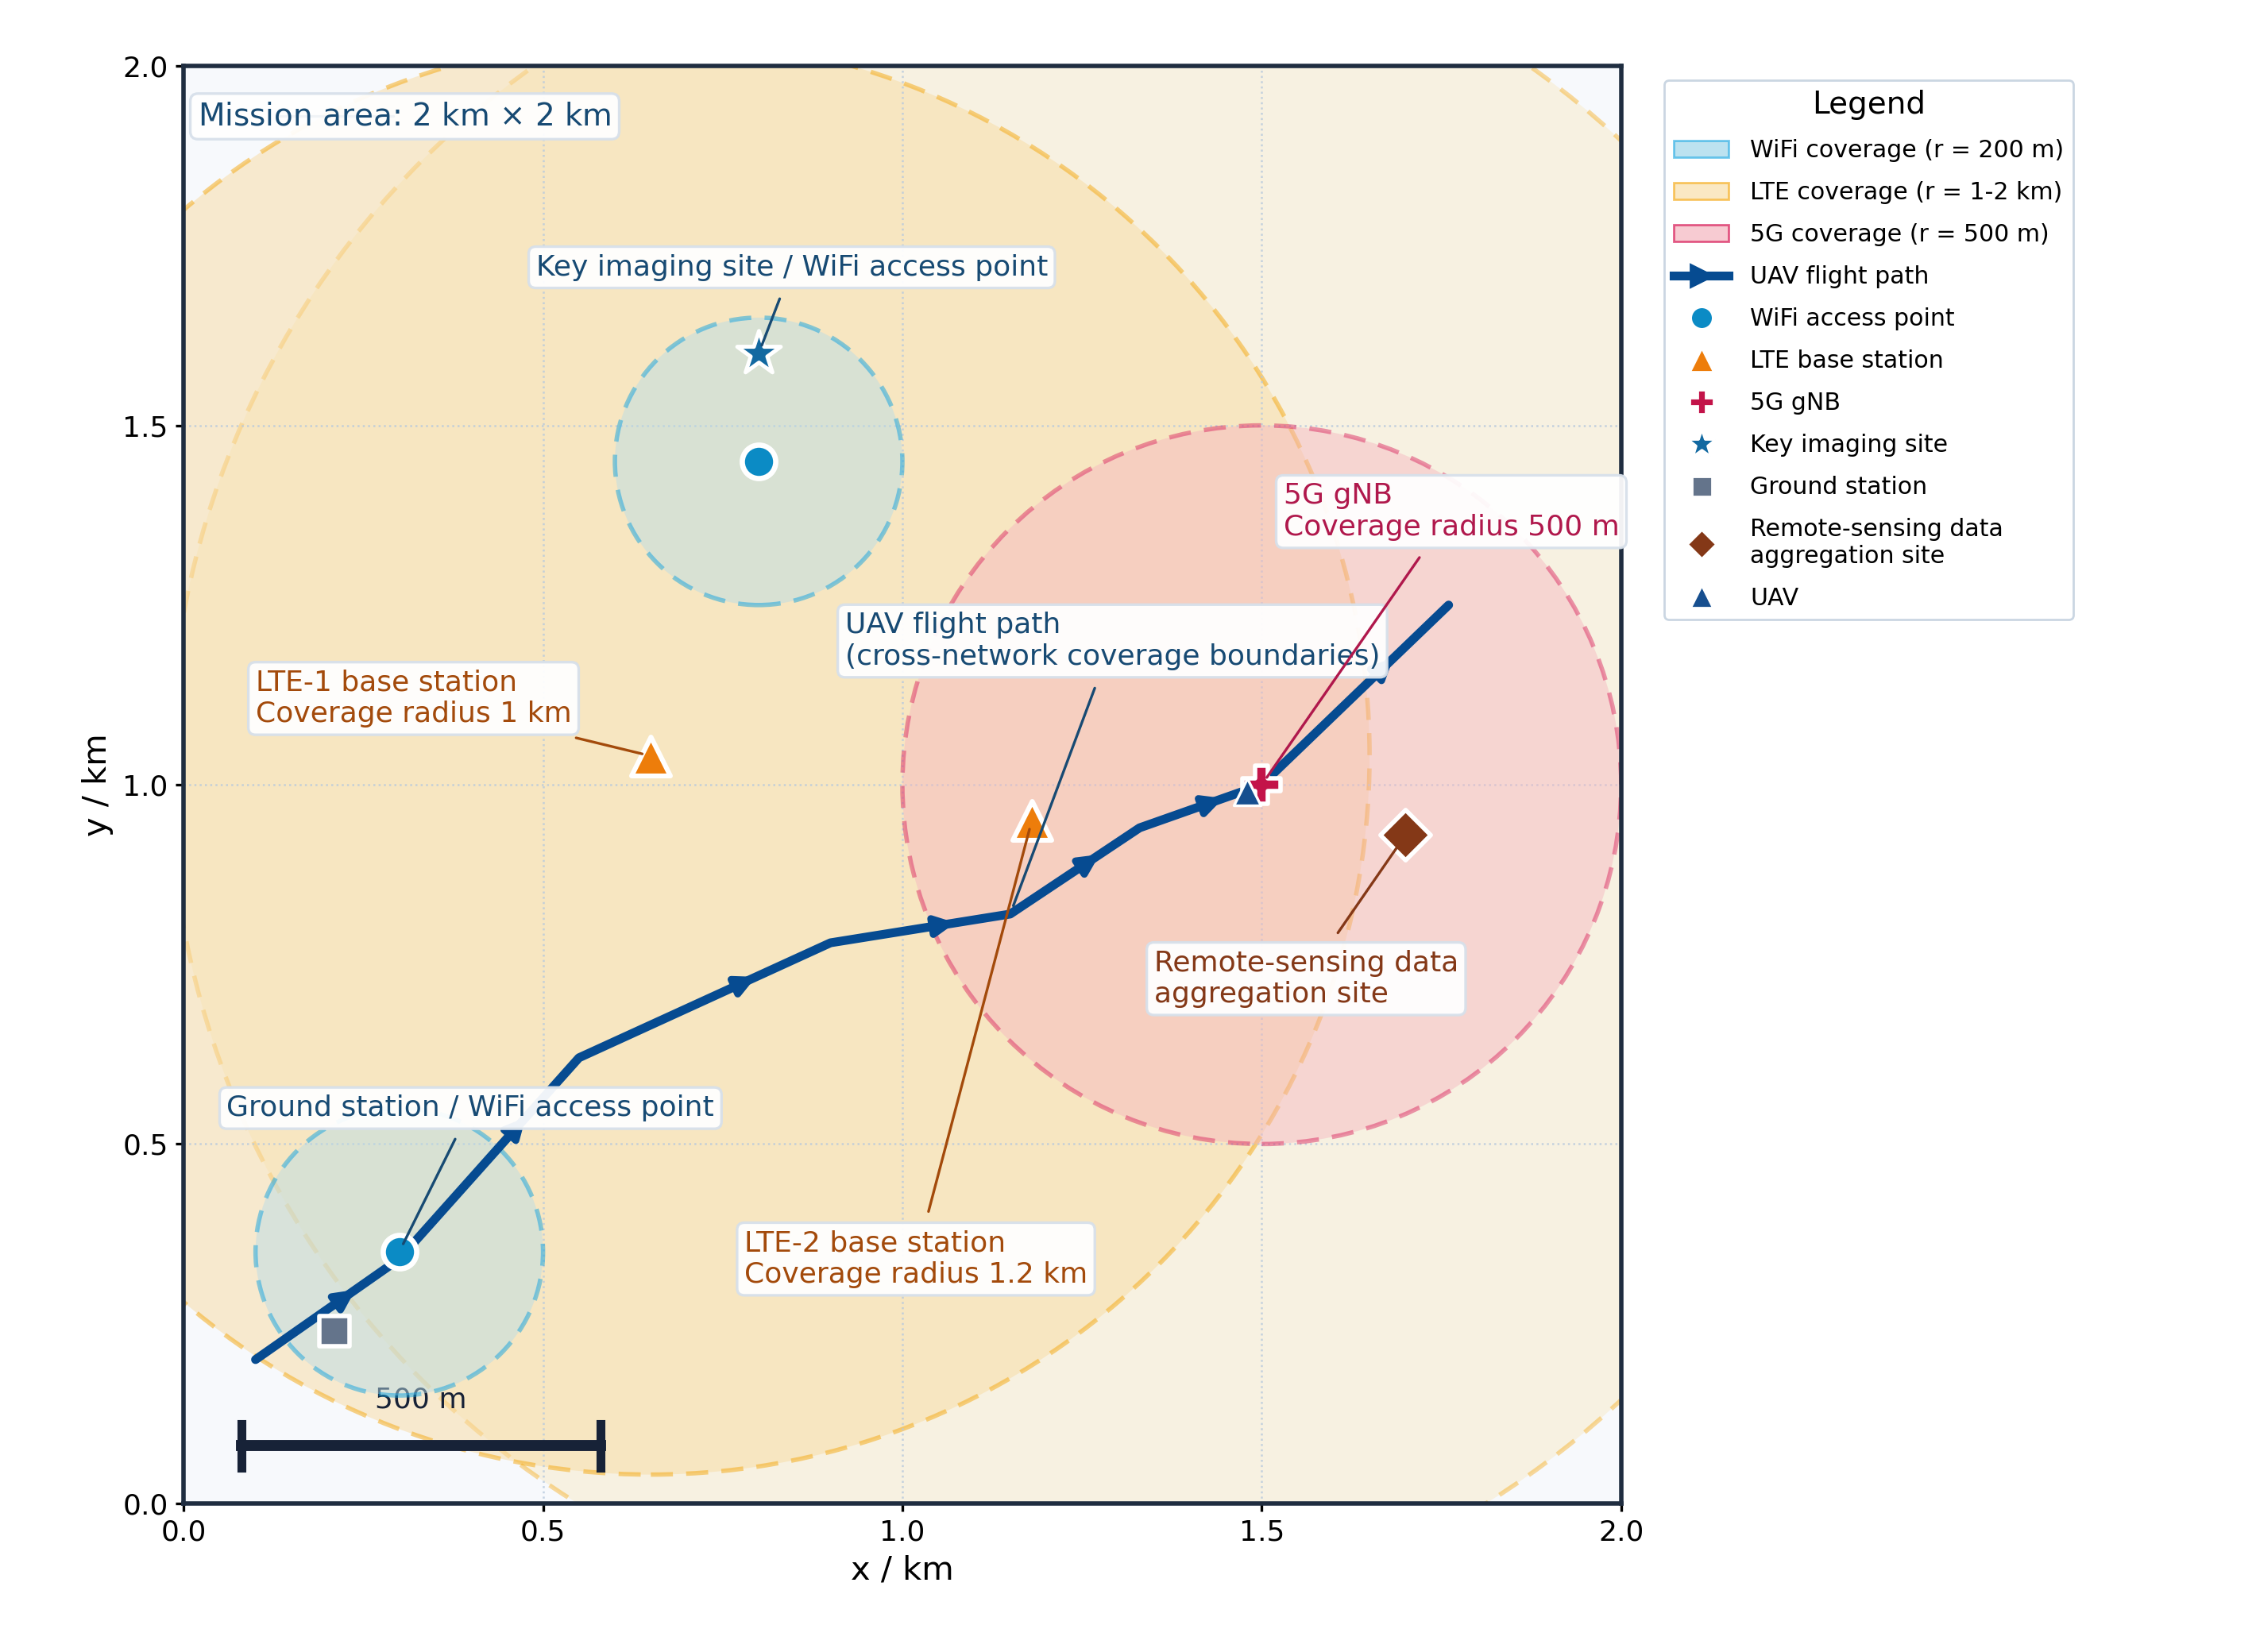
\includegraphics[width=\textwidth]{Figures/plots_chapter3_v2_en.png}
\caption{Heterogeneous wireless network coverage and UAV trajectory in the mission area.}
\label{fig:network_coverage}
\end{figure}

Wi-Fi, LTE, and 5G provide overlapping coverage at different scales (Figure~\ref{fig:network_coverage}). Wi-Fi hotspots mainly serve ground stations and key imaging sites; LTE base stations offer relatively continuous wide-area connectivity; and 5G base stations provide high-rate transmission within the eastern data-aggregation area but with limited coverage continuity. The 5G next generation Node B (gNB) provides 5G coverage, radio-resource scheduling, and high-rate data transmission. As the UAV follows its route, it traverses overlapping coverage areas and requires VHO when the serving network degrades; another candidate offers better overall performance. The coverage scales correspond to the specified radii and define the basis for subsequent network-state collection and candidate evaluation.

For candidate network $i$, the state vector at time $t$ is defined as:
\begin{equation}
S_i(t)=\left[\mathrm{SINR}_i(t),\,\mathrm{RSRP}_i(t),\,D_i(t),\,T_i(t),\,\mathrm{PLR}_i(t)\right],
\label{eq:state}
\end{equation}

where $\mathrm{SINR}_i(t)$, $\mathrm{RSRP}_i(t)$, $D_i(t)$, $T_i(t)$, and $\mathrm{PLR}_i(t)$ denote the SINR, reference signal received power, end-to-end delay, throughput, and packet loss ratio of candidate \textit{i} at time \textit{t}, respectively. These five indicators characterize candidate-network performance from complementary perspectives. As the UAV moves across coverage boundaries, $\mathrm{SINR}_i(t)$ typically declines from tens of decibels toward the noise floor, reflecting signal degradation caused by distance and obstruction and providing a direct handover cue. $\mathrm{RSRP}_i(t)$, together with $\mathrm{SINR}_i(t)$, determines whether the link budget meets the demodulation threshold; below receiver sensitivity, reliable physical-layer connectivity cannot be established even with acceptable SINR. The delay $D_i(t)$ represents the round-trip time of a packet between the ground station and UAV application layer, affecting responsiveness and safety margins during high-speed cruise. Throughput $T_i(t)$ measures deliverable payload bits per unit time; insufficient throughput prevents time-sensitive data payloads from being transmitted during a single overflight. While $\mathrm{PLR}_i(t)$ reflects transmission reliability, even with adequate signal strength and throughput, high $\mathrm{PLR}_i(t)$ can cause data loss or quality degradation. $\mathrm{SINR}_i(t)$, $\mathrm{RSRP}_i(t)$, and $T_i(t)$ are benefit criteria, whereas $D_i(t)$ and $\mathrm{PLR}_i(t)$ are cost criteria. Min-max normalization maps all indicators to $[0,1]$, where larger normalized values indicate better performance \cite{ref11}.

Equation~\eqref{eq:state} provides the common input interface for the subsequent algorithm chain. Stacking $S_i(t)$ for the three candidates at time \textit{t} forms the current-state matrix $S_{\mathrm{cur}}\in\mathbf{R}^{3\times5}$, which feeds the attention-based weight-generation module (Section~\ref{sec:weight}). Stacking one candidate's states over 10 consecutive decision periods forms the historical-state tensor $X_k\in\mathbf{R}^{10\times5}$, which feeds the stacked-LSTM prediction module (Section~\ref{sec:pred}). Therefore, the network-state parameters in Section~\ref{sec:scenario} capture both cross-candidate differences and the short-term evolution of individual networks induced by UAV mobility.

UAV motion continuously changes candidate signal and transmission performance. Relying only on current indicators may prevent timely handover near coverage edges, increasing link-interruption risk and degrading service continuity; UAV cellular-network coverage and handover characteristics are discussed in \cite{ref23}. Recent work has also investigated 5G ping-pong handover suppression through self-optimization \cite{ref24}. Accordingly, the algorithm uses network states from recent decision periods as temporal inputs to predict short-term future states and combines them with the current state for the final handover decision.

\section{LAAVHA Adaptive Vertical Handover Algorithm}\label{sec:laavha}

Based on the network scenario and state parameters (Section~\ref{sec:scenario}), this section proposes LAAVHA, an adaptive VHO algorithm that integrates LSTM and an attention mechanism. It overcomes the fixed weighting and lack of temporal prediction in conventional MADM methods for UAV aerial missions in heterogeneous wireless networks. Using the five-dimensional state vector and sliding window (Section~\ref{sec:scenario}), LAAVHA performs stacked-LSTM prediction, attention-based dynamic weighting, and improved TOPSIS decision-making with predicted states. ADH and RS-TOPSIS are then incorporated to form ALERA.

\begin{figure}[H]
\centering
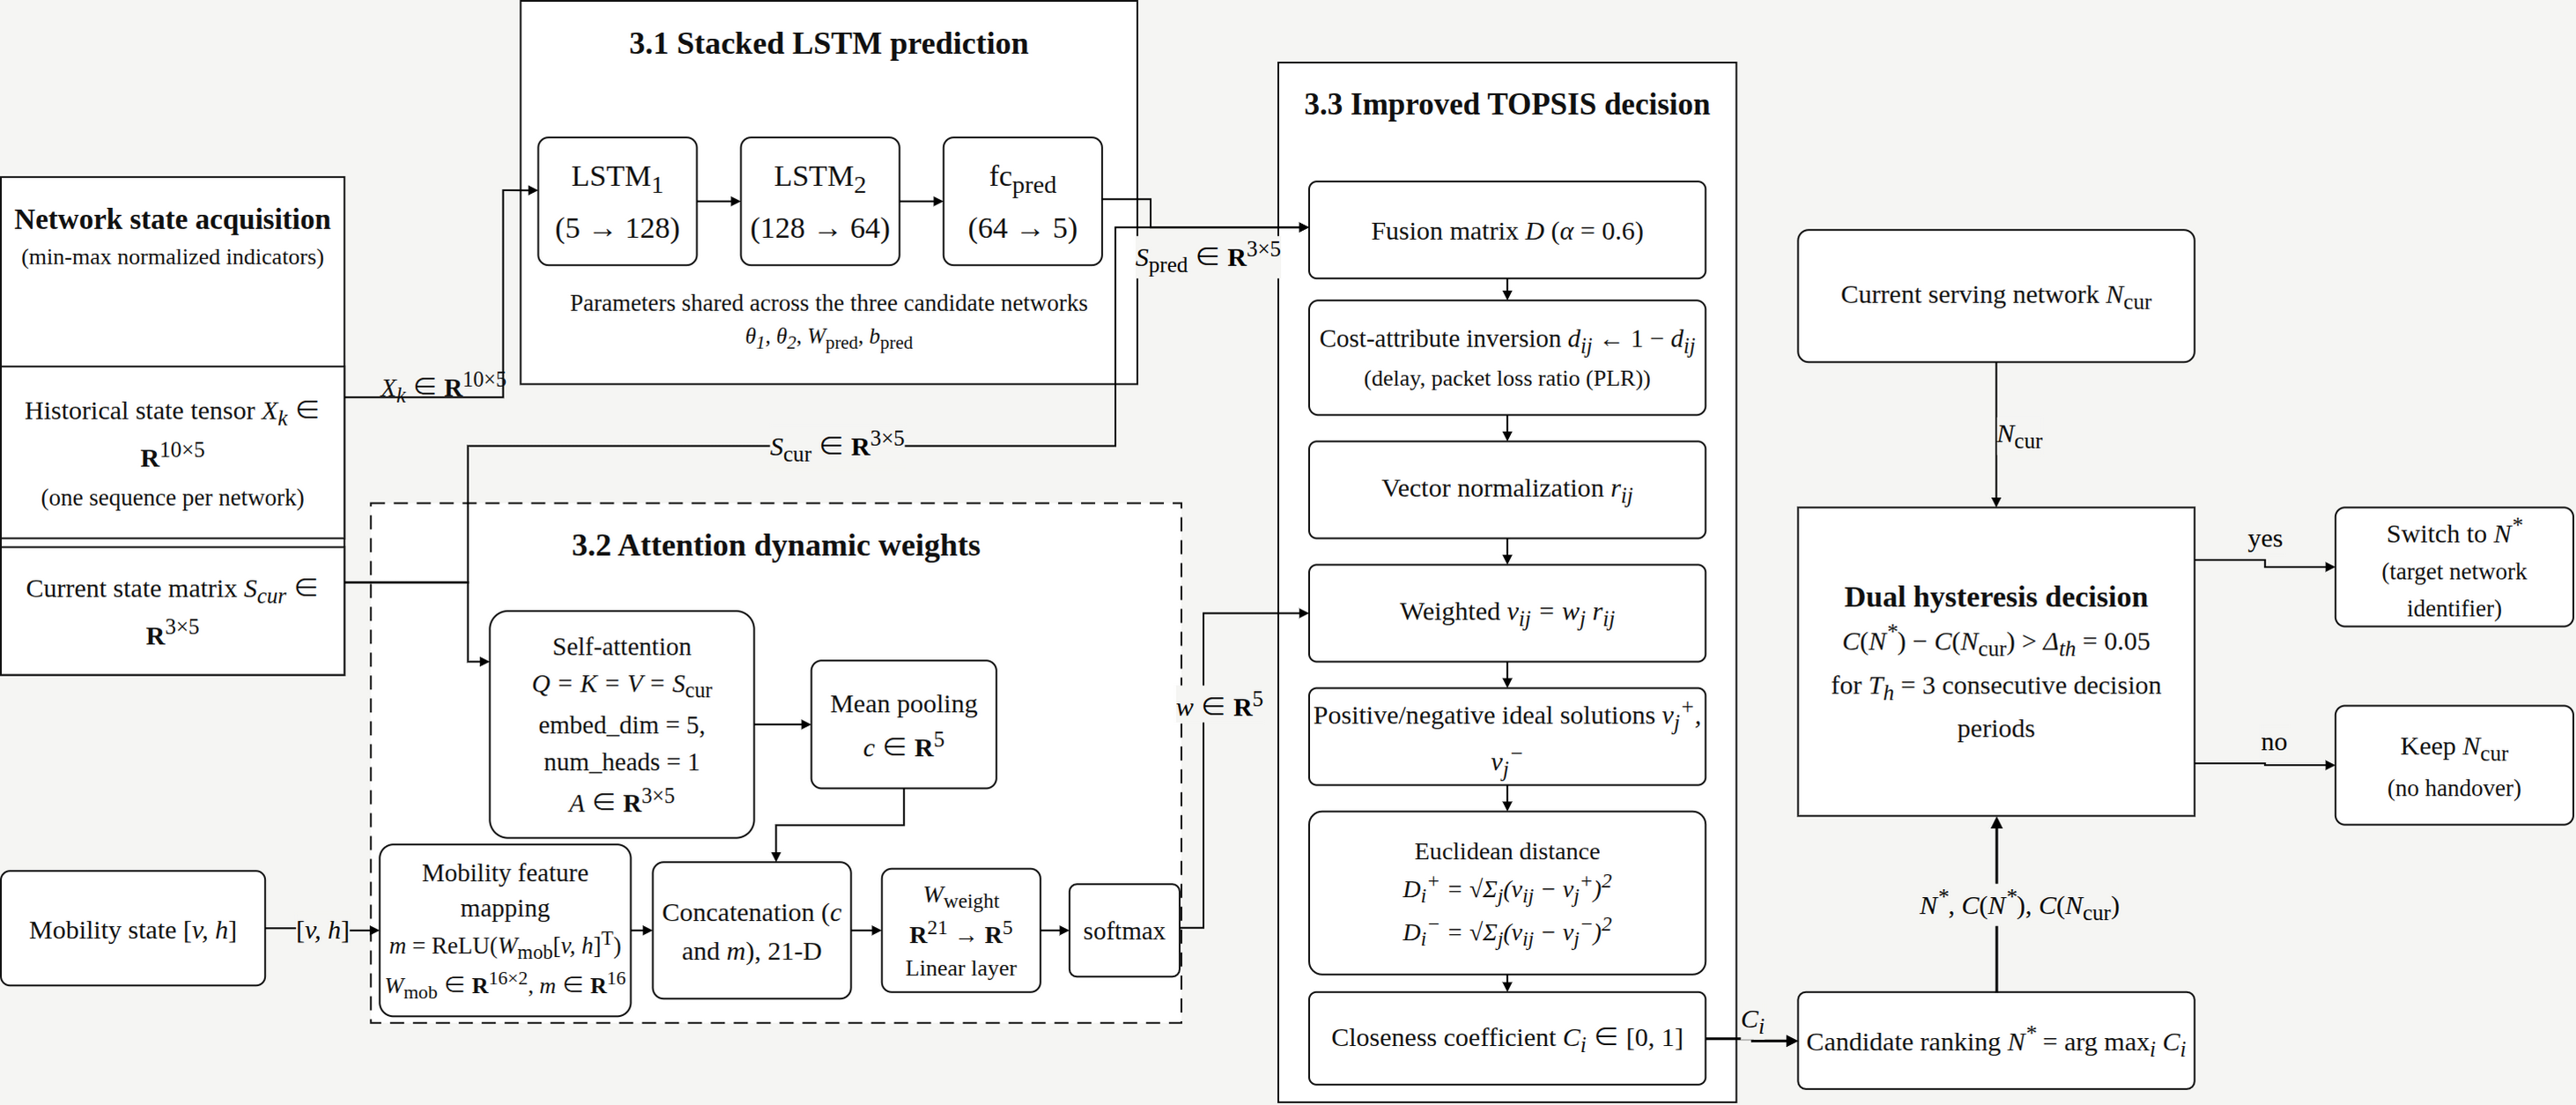
\includegraphics[width=\textwidth]{Figures/fig_laavha_framework_en.png}\\[1mm]
(a) LAAVHA algorithm framework\\[3mm]
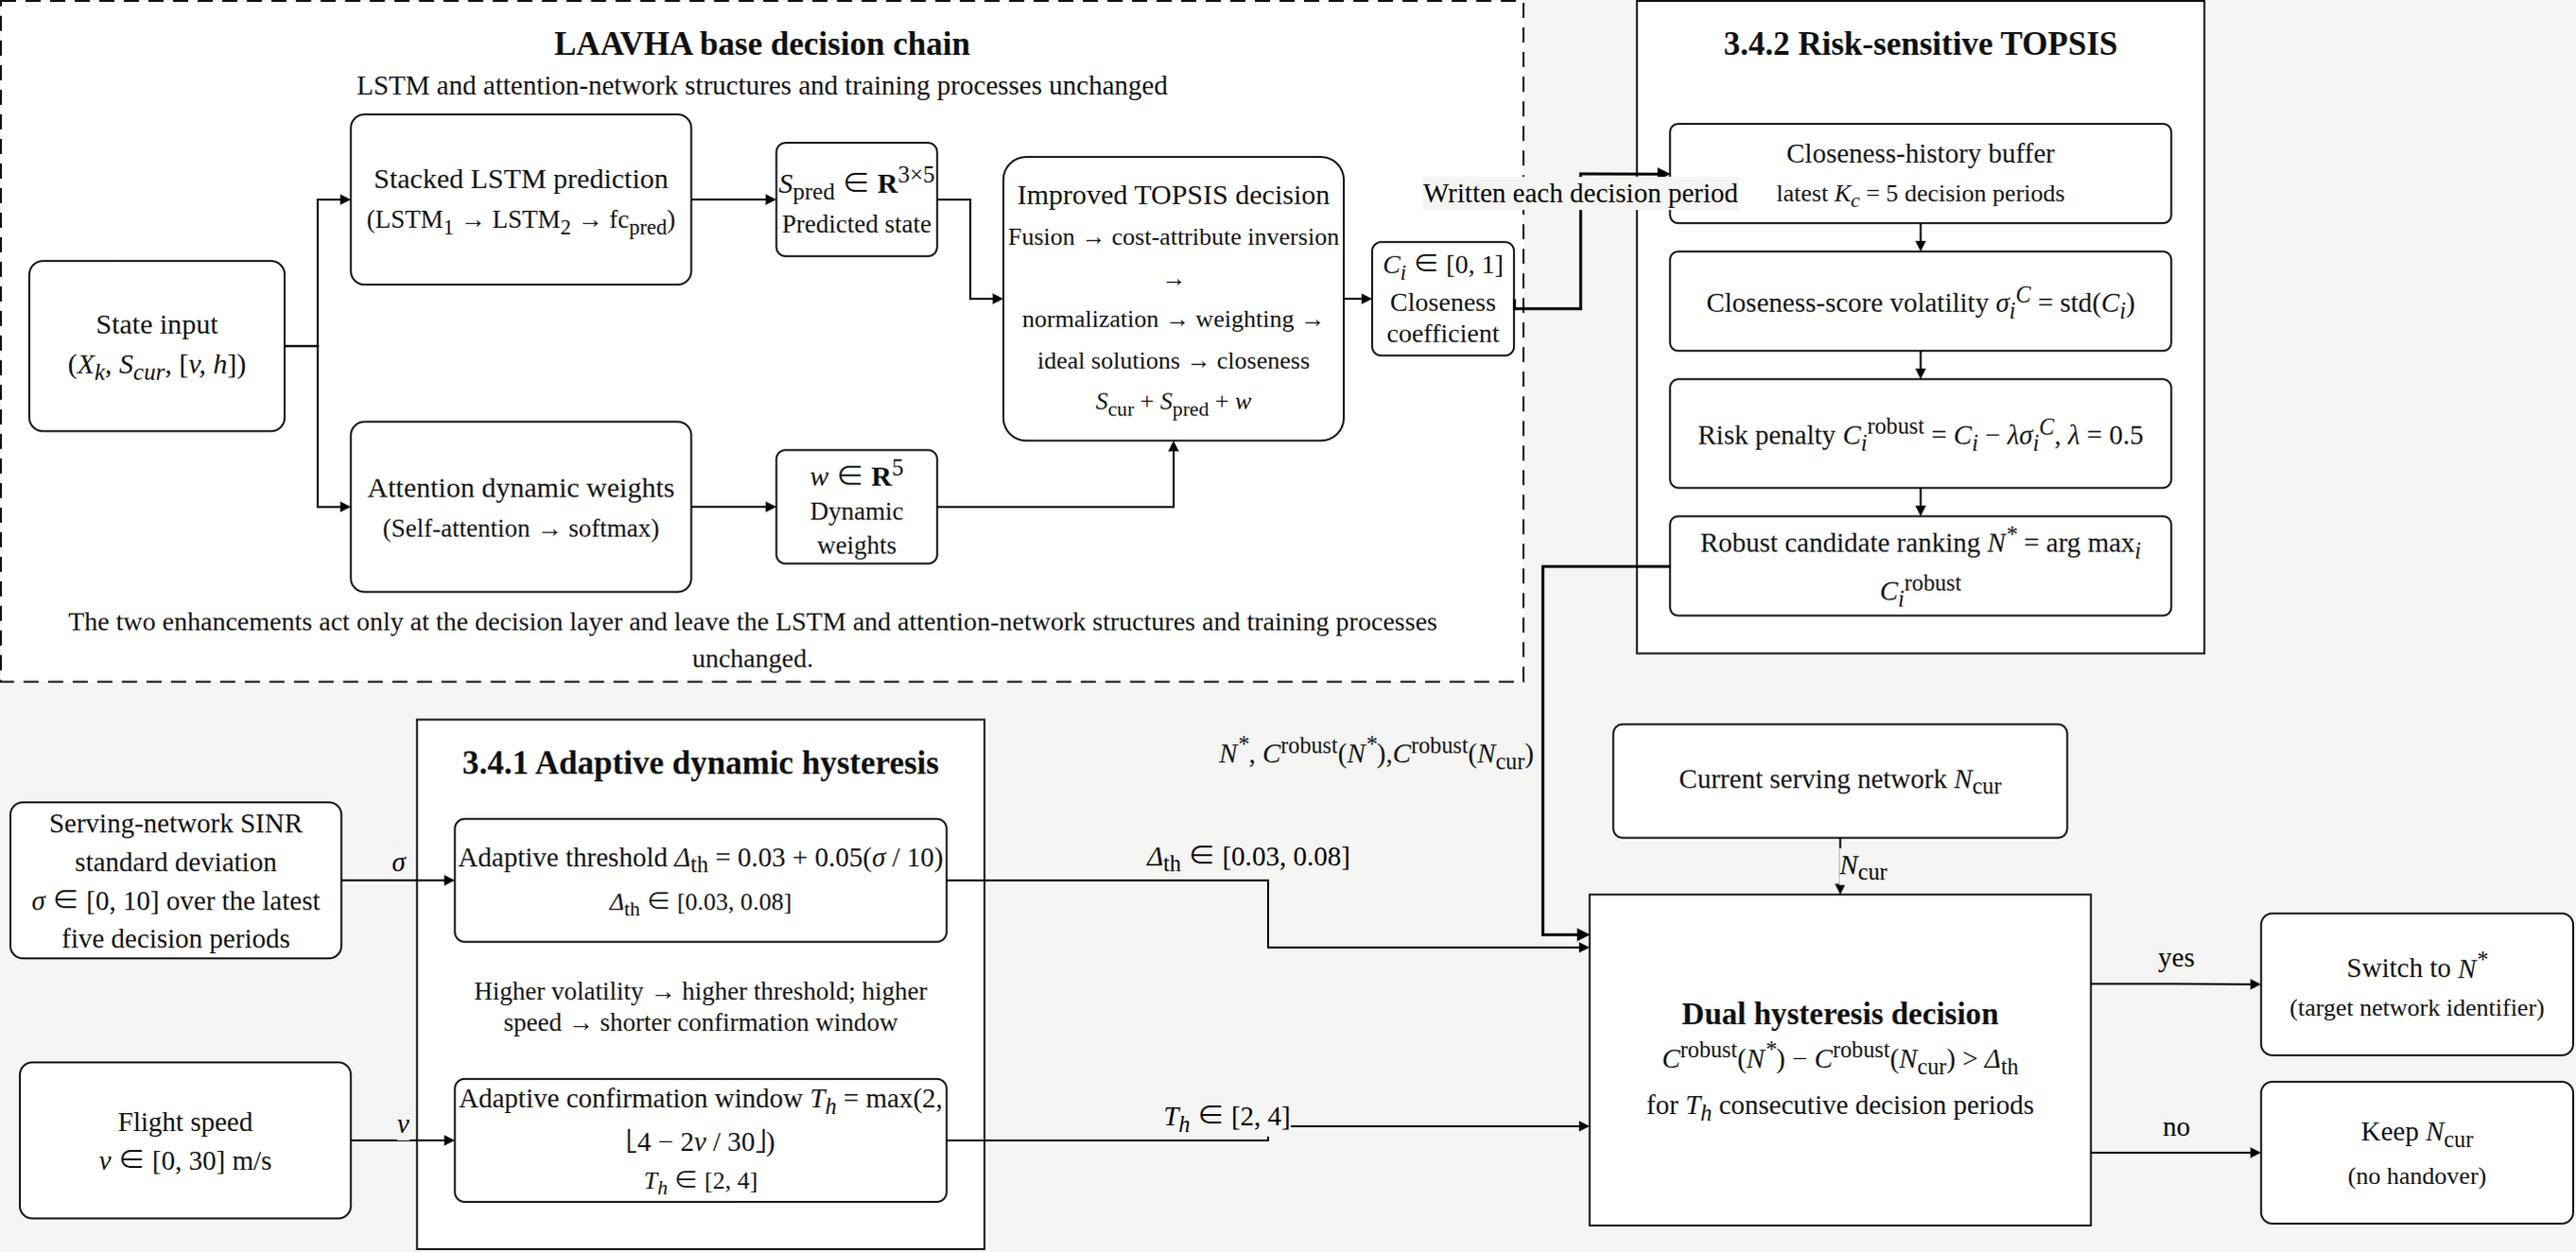
\includegraphics[width=\textwidth]{Figures/fig_alera_framework_en.png}\\[1mm]
(b) ALERA algorithm framework
\caption{LAAVHA and ALERA algorithm frameworks.}
\label{fig:frameworks}
\end{figure}

LAAVHA comprises network-state prediction, dynamic-weight generation, candidate ranking, and dual-hysteresis decision-making, with ADH and RS-TOPSIS extending the decision chain (Figure~\ref{fig:frameworks}). These modules form a sequential flow around a common network state. The historical sequence $X_k$, collected and normalized in Section~\ref{sec:scenario}, enters the stacked LSTM to produce the next-period predicted state $S_{\mathrm{pred}}$. Additionally, the current-state matrix $S_{\mathrm{cur}}$ enters the attention module with mobility features, including speed and altitude, to generate dynamic weight $w$. Then $S_{\mathrm{cur}}$, $S_{\mathrm{pred}}$, and $w$ are combined in improved TOPSIS to obtain candidate closeness score $C_i$. Finally, $C_i$ and the current serving network $N_{\mathrm{cur}}$ enter the hysteresis decision module with ALERA enhancements to determine the final handover. Therefore, Section~\ref{sec:pred} predicts future states, Section~\ref{sec:weight} determines attribute importance, Section~\ref{sec:topsis} ranks candidates using current and future states, and Section~\ref{sec:alera} determines whether handover is appropriate under channel fluctuations.

In the prediction branch, $\theta_1$ and $\theta_2$ denote the parameters of the two LSTM layers, while $W_{\mathrm{pred}}$ and $b_{\mathrm{pred}}$ represent the prediction-head weight and bias. In the attention branch, $Q$, $K$, and $V$ indicate the query, key, and value; $A$ signifies the attention output; $c$ corresponds to the mean-pooled context vector; $v$ and $h$ are flight speed and altitude; $W_{\mathrm{mob}}$ maps them to the mobility feature $m$; and $W_{\mathrm{weight}}$ projects the concatenated $c$ and $m$ to dynamic weight $w$. In the TOPSIS branch, $D$ represents the fused decision matrix; $\alpha$ denotes the fusion coefficient; $d_{ij}$, $r_{ij}$, and $v_{ij}$ denote the candidate's fused, normalized, and weighted elements, respectively; $v_j^+$ and $v_j^-$ indicate the positive and negative ideal solutions; $D_i^+$ and $D_i^-$ signify the Euclidean distances of candidate $i$ from these solutions; $C_i$ is its closeness score; $N^*$ corresponds to the selected target network; and $\Delta_{\mathrm{th}}$ and $T_h$ are the handover threshold and consecutive-confirmation window. In the enhancement branch, $K_c$ denotes the closeness-history length, $\sigma_i^C$ represents the standard deviation of candidate $i$'s scores, $\lambda$ indicates the risk coefficient, $C_i^{\mathrm{robust}}$ signifies the risk-adjusted score, and $\sigma$ is the serving network's SINR standard deviation over the latest five periods.

\subsection{Network-State Prediction using a Stacked LSTM}\label{sec:pred}

The time-window length is set to $T_s=10$, covering 10 consecutive decision periods over $1.0~\mathrm{s}$ with a decision interval of $\tau=0.1~\mathrm{s}$. Candidate networks $k\in\{1,2,3\}$ represent 5G, LTE, and Wi-Fi, respectively. The historical input tensor $X_k\in\mathbf{R}^{10\times5}$ is constructed by row-wise stacking the normalized five-dimensional state vectors across the 10 periods. The prediction target is the next-period state vector $\hat{s}_k(t+\tau)\in\mathbf{R}^5$:
\begin{align}
h_{1,k} &= \mathrm{LSTM}_1(X_k;\theta_1), && h_{1,k}\in\mathbf{R}^{10\times128}, \label{eq:lstm1}\\
h_{2,k} &= \mathrm{LSTM}_2(h_{1,k};\theta_2), && h_{2,k}\in\mathbf{R}^{10\times64}, \label{eq:lstm2}\\
\hat{s}_k(t+\tau) &= W_{\mathrm{pred}}h_{2,k}[-1]+b_{\mathrm{pred}}, && \hat{s}_k\in\mathbf{R}^5. \label{eq:lstm3}
\end{align}
where $\theta_1$ and $\theta_2$ denote the trainable parameters of the two LSTM layers, including the weights and biases of the input, forget, and output gates and cell states, while $W_{\mathrm{pred}}\in\mathbf{R}^{5\times64}$ and $b_{\mathrm{pred}}\in\mathbf{R}^5$ represent the fully connected prediction-head weight and bias, respectively, and $h_{2,k}[-1]$ indicates the final output of $\mathrm{LSTM}_2$. Equations~\eqref{eq:lstm1}--\eqref{eq:lstm3} define the prediction pipeline: 10 steps $\times$ 5 indicators $\rightarrow\mathrm{LSTM}_1(5\rightarrow128)\rightarrow\mathrm{LSTM}_2(128\rightarrow64)\rightarrow$fc\_pred($64\rightarrow5$). The three candidate networks share $\theta_1$, $\theta_2$, $W_{\mathrm{pred}}$, and $b_{\mathrm{pred}}$, while using their respective historical sequences $X_k$. The resulting predictions are stacked into $S_{\mathrm{pred}}\in\mathbf{R}^{3\times5}$, representing the next-period values of the five indicators for each network.

The prediction branch is trained using supervised learning with mean squared error (MSE) loss. Given training samples indexed by $n=1,\ldots,N$, where each sample comprises a historical sequence $X_k^{(n)}$ and the corresponding ground-truth next-period state $S_{\mathrm{target}}^{(n)}$, the loss function is:
\begin{equation}
\mathcal{L}_{\mathrm{pred}} = \frac{1}{N}\sum_{n=1}^{N}\left\|S_{\mathrm{pred}}^{(n)} - S_{\mathrm{target}}^{(n)}\right\|_2^2. \label{eq:loss_pred}
\end{equation}
The parameters $\theta_1$, $\theta_2$, $W_{\mathrm{pred}}$, and $b_{\mathrm{pred}}$ are updated via backpropagation using the Adam optimizer. Training uses an 80\%/20\% train/validation split with early stopping when validation loss does not decrease for 10 consecutive epochs. This supervised objective trains the LSTM branch to accurately forecast short-term network-state evolution, which subsequently feeds the TOPSIS decision module.

$S_{\mathrm{pred}}$ is not a direct handover score but a comparable prediction of each candidate's next-period state derived from its historical sequence $X_k$. In Section~\ref{sec:topsis}, Equation~\eqref{eq:fuse}, it is fused with the current state $S_{\mathrm{cur}}$, enabling TOPSIS to incorporate both current measurements and short-term predictions. Without $S_{\mathrm{pred}}$, handover decisions would rely solely on passive ranking of $S_{\mathrm{cur}}$, as evaluated by the LAAVHA-L ablation variant.

\subsection{Dynamic Weight Generation for Flight Phases}\label{sec:weight}

Network-attribute importance varies with the VHO decisions. During cruise, link stability and flight-control delay are more critical to safety, whereas during image return at imaging sites, throughput and packet loss become more important for timely and reliable transmission of high-resolution images \cite{ref25}. Fixed weights cannot capture these changing priorities.

To capture phase-dependent requirements, LAAVHA employs self-attention \cite{ref26,ref27}. The five-dimensional state vectors of the three candidates are row-wise stacked into $S_{\mathrm{cur}}\in\mathbf{R}^{3\times5}$, with $Q=K=V=S_{\mathrm{cur}}$, \texttt{embed\_dim} = 5, and \texttt{num\_heads} = 1. The \texttt{embed\_dim} denotes the feature dimension of each attention input and is set to 5, corresponding to the normalized SINR, RSRP, delay, throughput, and packet loss ratio indicators, and \texttt{num\_heads} represents the number of parallel attention heads and is set to 1. With five attributes, multiple heads would provide too few features per head and reduce weight interpretability. A single head therefore captures attribute correlations directly. The self-attention mechanism captures cross-network dependencies among the candidate networks, where the attention matrix quantifies how each network's state should be aggregated based on inter-network relationships. Cross-network mean pooling then extracts the attribute-level context $c\in\mathbf{R}^5$ from the attention output. The resulting representations are combined with UAV mobility features to generate dynamic attribute weights for subsequent TOPSIS-based network selection. Flight speed $v$ and altitude $h$ are mapped by $W_{\mathrm{mob}}\in\mathbf{R}^{16\times2}$ to mobility feature $m\in\mathbf{R}^{16}$. The concatenated results are projected by a fully connected layer and normalized by softmax to obtain the five-dimensional dynamic weight $w$:
\begin{align}
Q &= K = V = S_{\mathrm{cur}}\in\mathbf{R}^{3\times5}, \label{eq:attn1}\\
A &= \mathrm{Attention}(Q,K,V)=\mathrm{softmax}\!\left(\frac{QK^\top}{\sqrt{5}}\right)V,\quad A\in\mathbf{R}^{3\times5}, \label{eq:attn2}\\
c &= \mathrm{mean}(A,\mathrm{dim}=0)\in\mathbf{R}^5, \label{eq:attn3}\\
m &= \mathrm{ReLU}\!\left(W_{\mathrm{mob}}[v,h]^\top\right),\quad W_{\mathrm{mob}}:\mathbf{R}^{2}\rightarrow\mathbf{R}^{16},\quad m\in\mathbf{R}^{16}, \label{eq:attn4}\\
w &= \mathrm{softmax}\!\left(W_{\mathrm{weight}}[c\parallel m]\right),\quad W_{\mathrm{weight}}:\mathbf{R}^{21}\rightarrow\mathbf{R}^{5},\quad w\in\mathbf{R}^{5},\quad \sum_j w_j=1. \label{eq:attn5}
\end{align}
Equations~\eqref{eq:attn1}--\eqref{eq:attn5} define the dynamic-weight procedure: $S_{\mathrm{cur}}\in\mathbf{R}^{3\times5}$ enters self-attention, producing the $3\times5$ matrix $A$; cross-network mean pooling yields the five-dimensional attribute context $c$; $W_{\mathrm{mob}}:2\rightarrow16$ maps speed and altitude to the 16-dimensional mobility feature $m$; and their 21-dimensional concatenation is projected by $W_{\mathrm{weight}}$ and softmax-normalized to obtain the five-dimensional dynamic weight $w$. The self-attention mechanism does not directly model attribute-to-attribute correlations; instead, it captures cross-network dependencies in the state matrix $S_{\mathrm{cur}}$, and the subsequent mean pooling and projection layers (Equations~\eqref{eq:attn3}--\eqref{eq:attn5}) transform this network-level context into attribute-level weights $w$.

The output $w$ is not an independent assessment of a network quality measure but an input to the TOPSIS weighting step in Section~\ref{sec:topsis}. In Equation~\eqref{eq:topsis2}, $v_{ij}=w_jr_{ij}$ applies $w_j$ to the $j$th attribute of the fused matrix $D$, allowing the importance of SINR, RSRP, delay, throughput, and packet loss ratio to adapt to the current network and flight state. Therefore, the LSTM branch predicts future state changes, while the attention branch determines current attribute importance; both contribute to the final TOPSIS closeness score $C_i$.

Unlike the LSTM prediction branch, the attention-based weight-generation module is not trained via gradient descent. Its parameters (attention mechanism weights, $W_{\mathrm{mob}}$, and $W_{\mathrm{weight}}$) are initialized using standard PyTorch initialization schemes (Xavier uniform for linear layers) and remain fixed during training. The module functions as a deterministic feature extractor that transforms the current network state $S_{\mathrm{cur}}$ and mobility features $[v,h]$ into dynamic attribute weights $w$ through forward-pass computation only. Although the attention module's parameters remain fixed, the output weights $w=f(S_{\mathrm{cur}},v,h)$ dynamically vary as a function of the current network state and mobility features. As network conditions and flight phases evolve across decision periods, the same fixed transformation produces different attribute importances, enabling input-driven adaptivity rather than parameter-driven learning. This design trades end-to-end trainability for architectural simplicity while preserving the core benefit: context-aware weight adjustment without manual tuning. This design choice has two motivations. First, there is no ground-truth target for what the optimal attribute weights should be at each decision period; constructing such supervision would require domain expertise or iterative reward-based tuning. While reinforcement learning could optimize weights using handover-count-based rewards, our preliminary experiments showed that the fixed-initialization structure already achieves substantial improvement (Section~\ref{sec:ablation}), making the additional training complexity and data requirements unnecessary for the current performance target. Second, the attention mechanism's structural inductive bias---specifically, the query-key interaction (Equation~\eqref{eq:attn2}) naturally capturing attribute correlations and the mobility projection (Equations~\eqref{eq:attn4}--\eqref{eq:attn5}) adapting to flight phase---provides meaningful feature transformation even without gradient-based parameter updates, analogous to how carefully designed convolutional kernels can extract useful features before fine-tuning. Experimental results in Section~\ref{sec:ablation} demonstrate that this initialization-based weight generation, combined with trained LSTM prediction, achieves substantial handover reduction compared to fixed-weight baselines (2.13 vs. 24.25 for entropy weighting in the 250-trajectory ablation study), validating the effectiveness of the attention module's structural design even without end-to-end training.

\subsection{Improved TOPSIS Decision Making with Fused Predicted States}\label{sec:topsis}

This subsection integrates the preceding learning modules. $S_{\mathrm{pred}}$ from Section~\ref{sec:pred} provides the short-term future state, $w$ from Section~\ref{sec:weight} provides phase-dependent attribute weights, and $S_{\mathrm{cur}}$ from Section~\ref{sec:scenario} provides the current state. Since aerial mission performance depends jointly on signal strength, transmission capability, and reliability, no single indicator defines the optimal network. TOPSIS ranks candidates by their proximity to the virtual ideal and negative-ideal networks \cite{ref8,ref9}. To incorporate future conditions, LAAVHA fuses the current and predicted states to form the decision matrix:
\begin{align}
s_{\mathrm{norm}} &= \frac{s-s_{\min}}{s_{\max}-s_{\min}},\quad \text{for each indicator }j, \label{eq:norm}\\
d_{ij} &= \alpha s_{\mathrm{cur}}(i,j)+(1-\alpha)s_{\mathrm{pred}}(i,j),\quad \alpha=0.6, \label{eq:fuse}\\
d_{ij} &\leftarrow 1-d_{ij},\quad j\in\{\mathrm{delay},\mathrm{PLR}\}. \label{eq:cost}
\end{align}
where $i=1,2,3$ denotes the candidate network index for 5G, LTE, and Wi-Fi, respectively, $j$ represents the attribute index for SINR, RSRP, delay, throughput, and packet loss ratio, $s$ indicates the original attribute value, $s_{\min}$ and $s_{\max}$ are its minimum and maximum values across candidates in the current period, $s_{\mathrm{norm}}$ indicates the normalized value in $[0,1]$, $s_{\mathrm{cur}}(i,j)$ and $s_{\mathrm{pred}}(i,j)$ correspond to the normalized current and LSTM-predicted next-period values, respectively and $d_{ij}$ denotes the resulting fused element of decision matrix $D$. The fusion coefficient $\alpha=0.6$, justified experimentally in Section~\ref{sec:platform}, prioritizes current measurements while retaining predictive guidance. Delay and packet loss ratio are cost criteria; therefore, Equation~\eqref{eq:cost} inverts their normalized values so that all TOPSIS inputs follow a larger-is-better orientation. The resulting fused decision matrix $D\in\mathbf{R}^{3\times5}$ then enters standard TOPSIS:
\begin{align}
r_{ij} &= \frac{d_{ij}}{\sqrt{\sum_{k=1}^{3}d_{kj}^{2}}}, \label{eq:topsis1}\\
v_{ij} &= w_j r_{ij}, \label{eq:topsis2}\\
v_j^+ &= \max_i v_{ij},\quad v_j^-=\min_i v_{ij}, \label{eq:topsis3}\\
D_i^+ &= \sqrt{\sum_{j=1}^{5}(v_{ij}-v_j^+)^2},\quad
D_i^-=\sqrt{\sum_{j=1}^{5}(v_{ij}-v_j^-)^2}, \label{eq:topsis4}\\
C_i &= \frac{D_i^-}{D_i^+ + D_i^-},\quad C_i\in[0,1]. \label{eq:topsis5}
\end{align}
where $r_{ij}$ denotes the vector-normalized element of fused matrix $D$, and $\sqrt{\sum_{k=1}^{3}d_{kj}^{2}}$ represents the Euclidean norm of attribute $j$ across the three candidates, with $k$ as the summation index, $w_j$ indicates the dynamic weight of attribute $j$ from the attention module, $v_{ij}$ signifies the weighted normalized element, $v_j^+$ and $v_j^-$ correspond to the positive and negative ideal solutions, defined as the largest and smallest weighted normalized values for attribute $j$, respectively, $D_i^+$ and $D_i^-$ are the distances of candidate $i$ from these solutions, and $C_i\in[0,1]$ is its relative closeness. Therefore, Equations~\eqref{eq:topsis1}--\eqref{eq:topsis5} convert the $3\times5$ fused matrix into three closeness scores through normalization, dynamic weighting, ideal-solution determination, and Euclidean-distance calculation. A value closer to 1 indicates stronger overall support for image transmission, flight-control responsiveness, and link reliability.
\begin{align}
N^* &= \arg\max_i C_i, \label{eq:select}\\
\mathrm{Decision} &=
\begin{cases}
\text{switch to }N^*, & C(N^*)-C(N_{\mathrm{cur}})>\Delta_{\mathrm{th}}\ \text{and lasts }T_h\text{ consecutive cycles},\\
\text{keep }N_{\mathrm{cur}}, & \text{otherwise},
\end{cases} \label{eq:hysteresis}
\end{align}
where $N^*$ denotes the candidate with the highest current closeness, $N_{\mathrm{cur}}$ represents the serving network, $C(N^*)$ and $C(N_{\mathrm{cur}})$ indicate their respective TOPSIS closeness scores, $\Delta_{\mathrm{th}}$ specifies the required score advantage, and $T_h$ specifies its required persistence. This study sets $\Delta_{\mathrm{th}}=0.05$ and $T_h=3$ based on experiments in Section~\ref{sec:platform}. To suppress ping-pong handovers caused by transient fluctuations, handover occurs only when $N^*$ exceeds $N_{\mathrm{cur}}$ by more than $\Delta_{\mathrm{th}}=0.05$ for $T_h=3$ consecutive periods. Algorithm~\ref{alg:laavha} integrates prediction, dynamic-weight generation, TOPSIS ranking, and hysteresis adjudication into the LAAVHA procedure.

\begin{algorithm}[H]
\caption{LAAVHA vertical-handover decision procedure}
\label{alg:laavha}
\small
\begin{algorithmic}[1]
\Require Historical states $\{X_k\}_{k=1}^{3}$, current state $S_{\mathrm{cur}}$, mobility state $[v,h]$, serving network $N_{\mathrm{cur}}$, previous confirmed candidate $N_{\mathrm{cand}}$, and its consecutive count $q$
\Ensure Handover decision $\mathrm{Decision}$ and updated $N_{\mathrm{cur}}$, $N_{\mathrm{cand}}$, and $q$
\State \textbf{Stage 0: Initialization}
\State Read the current decision-period state and previous hysteresis state $N_{\mathrm{cand}}$, $q$
\State \textbf{Stage 1: State prediction and dynamic-weight generation}
\For{$k\gets1$ \textbf{to} $3$}
 \State $h_{1,k}\gets\mathrm{LSTM}_1(X_k;\theta_1)$, $h_{2,k}\gets\mathrm{LSTM}_2(h_{1,k};\theta_2)$
 \State $s_{\mathrm{pred},k}\gets W_{\mathrm{pred}}h_{2,k}[-1]+b_{\mathrm{pred}}$
\EndFor
\State Stack $\{s_{\mathrm{pred},k}\}_{k=1}^{3}$ as $S_{\mathrm{pred}}$
\State $A\gets\mathrm{Attention}(S_{\mathrm{cur}},S_{\mathrm{cur}},S_{\mathrm{cur}})$, $c\gets\mathrm{mean}(A,\mathrm{dim}=0)$
\State $m\gets\mathrm{ReLU}(W_{\mathrm{mob}}[v,h]^\top)$, $w\gets\mathrm{softmax}(W_{\mathrm{weight}}[c\parallel m])$
\State \textbf{Stage 2: Fused-TOPSIS candidate ranking}
\For{$i\gets1$ \textbf{to} $3$}
 \For{$j\gets1$ \textbf{to} $5$}
 \State $d_{ij}\gets0.6s_{\mathrm{cur}}(i,j)+0.4s_{\mathrm{pred}}(i,j)$
 \If{$j\in\{\mathrm{delay},\mathrm{PLR}\}$} $d_{ij}\gets1-d_{ij}$ \EndIf
 \EndFor
\EndFor
\State Compute $r_{ij}$, $v_{ij}$, $v_j^+$, $v_j^-$, $D_i^+$, $D_i^-$, and $C_i$ using Equations~\eqref{eq:topsis1}--\eqref{eq:topsis5}
\State $N^*\gets\arg\max_i C_i$
\State \textbf{Stage 3: Dual-hysteresis handover decision}
\If{$N^*\ne N_{\mathrm{cand}}$}
 \State $N_{\mathrm{cand}}\gets N^*$, $q\gets0$
\EndIf
\If{$C(N^*)-C(N_{\mathrm{cur}})>\Delta_{\mathrm{th}}$}
 \State $q\gets q+1$
\Else
 \State $q\gets0$
\EndIf
\If{$q\geq T_h$}
 \State $\mathrm{Decision}\gets\text{switch to }N^*$, $N_{\mathrm{cur}}\gets N^*$
\Else
 \State $\mathrm{Decision}\gets\text{keep }N_{\mathrm{cur}}$
\EndIf
\State \Return $\mathrm{Decision}$, $N_{\mathrm{cur}}$, $N_{\mathrm{cand}}$, $q$
\end{algorithmic}
\end{algorithm}

Algorithm~\ref{alg:laavha} shows that the stacked LSTM generates only the predicted state $S_{\mathrm{pred}}$, while the attention module generates only the dynamic weight $w$. Both are combined with $S_{\mathrm{cur}}$ in TOPSIS to compute $C_i$, followed by dual hysteresis for the handover decision. The sequence follows Equations~\eqref{eq:lstm1}--\eqref{eq:hysteresis}.

\subsection{ALERA Enhanced Risk-Aware Vertical Handover Algorithm}\label{sec:alera}

Section~\ref{sec:topsis} establishes the base decision chain from state prediction and dynamic weighting to candidate ranking and handover, but its dual hysteresis uses fixed parameters. Although effective in stable channels, fixed thresholds and windows cannot balance fluctuation resistance and handover timeliness during coverage-boundary crossings, obstruction, or major speed changes. Standard TOPSIS also ranks candidates by current closeness without accounting for score-series risk. Without retraining the LSTM-attention model, this section introduces ADH and RS-TOPSIS. ADH uses serving-network SINR history and flight speed to dynamically update $\Delta_{\mathrm{th}}$ and $T_h$ in Equation~\eqref{eq:hysteresis}, while RS-TOPSIS uses the $C_i$ sequence from Section~\ref{sec:topsis} to derive risk-penalized $C_i^{\mathrm{robust}}$ for final candidate ranking, forming ALERA.

\subsubsection{Adaptive Hysteresis Parameters}\label{sec:adh}

Adaptive hysteresis margins and trigger windows improve handover decisions in heterogeneous and ultra-dense networks \cite{ref28,ref29,ref30,ref31}. Accordingly, fixed $\Delta_{\mathrm{th}}$ and $T_h$ are replaced with context-aware values. The variable $\sigma$ denotes the standard deviation of serving network SINR over the latest five decision periods, while $v$ denotes real-time flight speed, and $\sigma$ is derived from the SINR history in Equation~\eqref{eq:state}, and $v$ is the mobility input used for dynamic weighting in Section~\ref{sec:weight}. ADH thus reuses available states and adapts only the threshold and confirmation window of the final hysteresis decision. The adaptive threshold and window are:
\begin{align}
\Delta_{\mathrm{th}} &= 0.03+0.05\left(\frac{\sigma}{10}\right),\quad \sigma\in[0,10], \label{eq:adh1}\\
T_h &= \max\left(2,\left\lfloor4-\frac{2v}{30}\right\rfloor\right),\quad v\in[0,30]~\mathrm{m/s}. \label{eq:adh2}
\end{align}
Equation~\eqref{eq:adh1} sets a base threshold of 0.03 under stable channels ($\sigma\approx0$), below the fixed value of 0.05 and allowing faster response to sustained degradation. Under severe variation ($\sigma\approx10$), it increases linearly to 0.08, strengthening the handover barrier. Equation~\eqref{eq:adh2} sets a window of 4 at low speed ($v\approx5~\mathrm{m/s}$) for sufficient confirmation and decreases it to a minimum of 2 as speed increases, enabling timely handover near coverage boundaries. Therefore, $\Delta_{\mathrm{th}}\in[0.03,0.08]$ and $T_h\in[2,4]$ retain anti-chattering capability under extreme conditions. At $30~\mathrm{m/s}$, the UAV travels $3~\mathrm{m}$ in a $0.1~\mathrm{s}$ period; $T_h=4$ therefore permits $12~\mathrm{m}$ of movement, potentially shifting the UAV from Wi-Fi-center to edge coverage before confirmation. $T_h=2$ limits this to $6~\mathrm{m}$ and better supports boundary handover. At $5~\mathrm{m/s}$, $T_h=4$ corresponds to only $2~\mathrm{m}$, allowing longer confirmation to filter transient variations with limited obsolescence risk. The settings of $\Delta_{\mathrm{th}}$, $T_h$, and the $\sigma$ history length are validated experimentally in Section~\ref{sec:platform}.

\subsubsection{Risk-Sensitive TOPSIS}\label{sec:rstopsis}

Original TOPSIS ranks candidates by current closeness $C_i$, obtained from Equation~\eqref{eq:topsis5} by fusing $S_{\mathrm{cur}}$, $S_{\mathrm{pred}}$, and $w$. RS-TOPSIS retains this prediction and weighting process while adding a risk constraint to the $C_i$ series. Based on the lower-confidence-bound (LCB) principle, a historical-variation penalty is subtracted from each candidate score:
\begin{equation}
C_i^{\mathrm{robust}}=C_i-\lambda\sigma_i^C,\quad \lambda=0.5,
\label{eq:rstopsis}
\end{equation}
where $\sigma_i^C$ denotes the standard deviation of the latest five scores for network $i$, and $\lambda=0.5$ is the risk-aversion coefficient, justified experimentally in Section~\ref{sec:platform}. When current scores are similar, the mechanism favors the more stable candidate over one with a slightly higher mean but greater variation. For example, if LTE closeness increases steadily with low variance while Wi-Fi closeness fluctuates sharply, $C_i^{\mathrm{robust}}$ favors LTE even with slightly higher current Wi-Fi closeness, improving service continuity.

The two enhancements require no LSTM-attention retraining or changes to its inference structure. They apply lightweight statistical and rule-based updates to existing state and score sequences, adding minimal overhead to stacked-LSTM prediction and attention-weight generation. ADH adjusts the handover barrier based on channel variation and speed, while RS-TOPSIS reduces the ranking advantage of volatile candidates. Their impact is limited under stable channels but increases with variation, jointly strengthening environmental awareness and ping-pong suppression at low additional cost.

Algorithm~\ref{alg:alera} enhances the base closeness score at each decision period. Its $C_i$ input comes from Algorithm~\ref{alg:laavha}'s TOPSIS steps. RS-TOPSIS first adjusts the ranking score, ADH then updates the dual-hysteresis parameters, and the final decision remains dependent on persistent robust-score advantage.

\begin{algorithm}[H]
\caption{ALERA risk-aware vertical-handover enhancement procedure}
\label{alg:alera}
\small
\begin{algorithmic}[1]
\Require Base closeness $\{C_i\}_{i=1}^{3}$ and its latest $K_c=5$ history, latest five serving-network SINR values, flight speed $v$, serving network $N_{\mathrm{cur}}$, previous confirmed candidate $N_{\mathrm{cand}}$, and its consecutive count $q$
\Ensure Enhanced handover decision $\mathrm{Decision}$ and updated $N_{\mathrm{cur}}$, $N_{\mathrm{cand}}$, and $q$
\State \textbf{Stage 0: Initialize states and history cache}
\State Read base closeness, SINR history, speed, and previous hysteresis state $N_{\mathrm{cand}}$, $q$
\State \textbf{Stage 1: RS-TOPSIS risk-sensitive ranking}
\For{$i\gets1$ \textbf{to} $3$}
 \State Write $C_i$ to the closeness-history cache and retain the latest $K_c$ periods
 \State $\sigma_i^C\gets\mathrm{std}(\text{latest }K_c\text{-period history of }C_i)$
 \State $C_i^{\mathrm{robust}}\gets C_i-0.5\sigma_i^C$
\EndFor
\State $N^*\gets\arg\max_i C_i^{\mathrm{robust}}$
\State \textbf{Stage 2: ADH adaptive-hysteresis parameter update}
\State $\sigma\gets\mathrm{std}(\text{latest five SINR values of }N_{\mathrm{cur}})$
\State $\Delta_{\mathrm{th}}\gets0.03+0.05(\sigma/10)$, $T_h\gets\max(2,\lfloor4-2v/30\rfloor)$
\State \textbf{Stage 3: Robust-score dual-hysteresis decision}
\If{$N^*\ne N_{\mathrm{cand}}$}
 \State $N_{\mathrm{cand}}\gets N^*$, $q\gets0$
\EndIf
\If{$C^{\mathrm{robust}}(N^*)-C^{\mathrm{robust}}(N_{\mathrm{cur}})>\Delta_{\mathrm{th}}$}
 \State $q\gets q+1$
\Else
 \State $q\gets0$
\EndIf
\If{$q\geq T_h$}
 \State $\mathrm{Decision}\gets\text{switch to }N^*$, $N_{\mathrm{cur}}\gets N^*$
\Else
 \State $\mathrm{Decision}\gets\text{keep }N_{\mathrm{cur}}$
\EndIf
\State \Return $\mathrm{Decision}$, $N_{\mathrm{cur}}$, $N_{\mathrm{cand}}$, $q$
\end{algorithmic}
\end{algorithm}

\subsection{Complexity Analysis and Algorithm Summary}\label{sec:complexity}

Table~\ref{tab:complexity} summarizes the inputs, outputs, core procedures, and computational complexity of LAAVHA and ALERA in data-flow order. The stacked-LSTM prediction module (Section~\ref{sec:pred}) processes the historical state tensor $X_k\in\mathbf{R}^{10\times5}$ through two LSTM layers to generate $S_{\mathrm{pred}}\in\mathbf{R}^{3\times5}$, with gate-matrix computation as the bottleneck and complexity $O(R\cdot K\cdot d\cdot h^2)$. The dynamic-attention module (Section~\ref{sec:weight}) processes $S_{\mathrm{cur}}\in\mathbf{R}^{3\times5}$, incorporates mobility features, and outputs $w\in\mathbf{R}^5$, with self-attention complexity $O(R^2\cdot d)$. Improved TOPSIS (Section~\ref{sec:topsis}) fuses and normalizes $S_{\mathrm{cur}}$ and $S_{\mathrm{pred}}$, then ranks candidates using weights, producing $C_i$ with overall complexity $O(R\cdot d)$. ADH and RS-TOPSIS use SINR, speed, and $C_i$ history for lightweight statistical updates. End-to-end inference is dominated by LSTM prediction and attention-weight generation, supporting real-time handover decisions in UAV aerial mission scenarios in heterogeneous wireless networks.

\begin{table}[H]
\centering
\caption{Summary of the algorithms.}
\small
\begin{tabularx}{\textwidth}{>{\raggedright\arraybackslash}p{2.6cm}>{\raggedright\arraybackslash}X>{\raggedright\arraybackslash}X>{\raggedright\arraybackslash}p{2.3cm}}
\toprule
\textbf{Module} & \textbf{Input/output} & \textbf{Core procedure} & \textbf{Complexity} \\
\midrule
Stacked-LSTM prediction & In: $3\times10\times5$ state tensor; out: predicted state & $\mathrm{LSTM}_1(5\rightarrow128)\rightarrow\mathrm{LSTM}_2(128\rightarrow64)\rightarrow$fc($64\rightarrow5$) & $O(R\cdot K\cdot d\cdot h^2)$ \\
Attention dynamic weights & In: $3\times5$ state matrix + mobility features; out: 5-D dynamic weights & Self-Attn\arw{}mean pooling\arw{}concatenate mobility features\arw{}softmax & $O(R^2\cdot d)$ \\
Improved TOPSIS & In: current + predicted states + dynamic weights; out: candidate closeness $C_i$ & Fused matrix\arw{}weighted normalization\arw{}positive/negative ideal solutions\arw{}closeness & $O(R\cdot d)$ \\
ADH & In: SINR history + flight speed; out: adaptive $\Delta_{\mathrm{th}},T_h$ & SINR-variation calculation\arw{}linear threshold adjustment\arw{}window adaptation & $O(1)$ \\
RS-TOPSIS & In: recent closeness history; out: LCB-adjusted ranking & Historical standard deviation\arw{}penalty calculation$\rightarrow C_i^{\mathrm{robust}}$ ranking & $O(R\cdot K_c)$ \\
\bottomrule
\end{tabularx}
\label{tab:complexity}
\end{table}

\section{Simulation Experiments and Results Analysis}\label{sec:sim}

\subsection{Experimental Platform and Parameter Settings}\label{sec:platform}

To evaluate LAAVHA/ALERA in UAV heterogeneous wireless networks, a simulation and inference platform was developed using ns-3.45 \cite{ref32} and its AI extension ns3-ai \cite{ref33}. ns-3 implements the 5G/LTE/Wi-Fi topology, UAV mobility, and physical- and transport-layer measurements, while ns3-ai enables bidirectional simulation-inference communication through shared memory. Each decision period transfers a 10-step history of five indicators for three candidate networks (150 dimensions) and the mobility state to shared memory. The inference module loads the trained LAAVHA model, reads the network state, speed, altitude, and current-network identifier, and returns the target-network identifier and candidate scores. Network identifiers are 0=5G, 1=LTE, and 2=Wi-Fi. The model input comprises five indicators for each candidate network ($3$ networks $\times10$ time steps $\times5$ indicators = 150 dimensions), with each network processed independently by the stacked LSTM. Mobility input comprises speed and altitude. The model outputs a five-dimensional predicted state and dynamic weight, followed by candidate scoring through improved TOPSIS. The testing dataset uses seeds 200--449 (250 trajectories for algorithm comparison; the first 50 seeds, 200--249, are also used for ablation and QoS experiments). Each simulation lasts $50~\mathrm{s}$ with a $0.1~\mathrm{s}$ decision period, yielding 500 decisions per trajectory. Position and altitude perturbations of $30~\mathrm{m}$ and $10~\mathrm{m}$, respectively, represent flight deviations.

Before finalizing the parameters in Section~\ref{sec:laavha}, three sensitivity experiments were conducted, with results shown in Figure~\ref{fig:param_sensitivity}. The fusion-coefficient experiment replayed 50 stress sequences involving sustained link degradation and transient fluctuations. Current observations included channel-measurement variation, while predicted states exhibited short-term lag under abrupt changes. For $\alpha=0.2,0.4,0.6,0.8$, mean false-handover counts were 1.20, 0.90, 0.08, and 1.00, respectively. Lower $\alpha$ increased sensitivity to prediction lag, whereas higher $\alpha$ increased sensitivity to measurement variation. Therefore, $\alpha=0.6$ provided the best balance, minimizing false handovers and assigning 60\% weight to current measurements and 40\% to predictions.

Dual-hysteresis and enhancement parameters were evaluated over 50 repetitions of the two competitive intervals used in the subsequent scenario-adaptation experiment: sustained link degradation requiring handover and transient fluctuations that should not trigger handover. Across $\Delta_{\mathrm{th}}\in\{0.03,0.05,0.07\}$ and $T_h\in\{2,3,4\}$, all combinations achieved 100\% necessary-handovers. The $\Delta_{\mathrm{th}}=0.05,T_h=3$ setting yielded 0.64 mean false handovers and $1.55~\mathrm{s}$ mean detection delay. The more aggressive $0.03,2$ setting responded faster but produced 9.10 mean false handovers, whereas the conservative $0.07,4$ setting eliminated false handovers but increased mean detection delay to $2.00~\mathrm{s}$. Therefore, $0.05,3$ was selected to balance stability and response time.

The enhancement parameters $K_c\in\{3,5,7\}$ and $\lambda\in\{0.2,0.5,0.8\}$ were further evaluated, with all combinations identifying 100\% of necessary handovers. At $K_c=5$, increasing $\lambda$ from 0.2 to 0.8 reduced mean false handovers from 1.90 to 0.58 but increased mean detection delay from $1.13~\mathrm{s}$ to $1.22~\mathrm{s}$. At $\lambda=0.5$, $K_c=5$ produced 1.08 mean false handovers, compared with 1.48 for $K_c=3$ and 1.14 for $K_c=7$, with a mean detection delay of $1.17~\mathrm{s}$. Considering risk suppression, history stability, and handover timeliness, $K_c=5,\lambda=0.5$ were selected.

\begin{figure}[H]
\centering
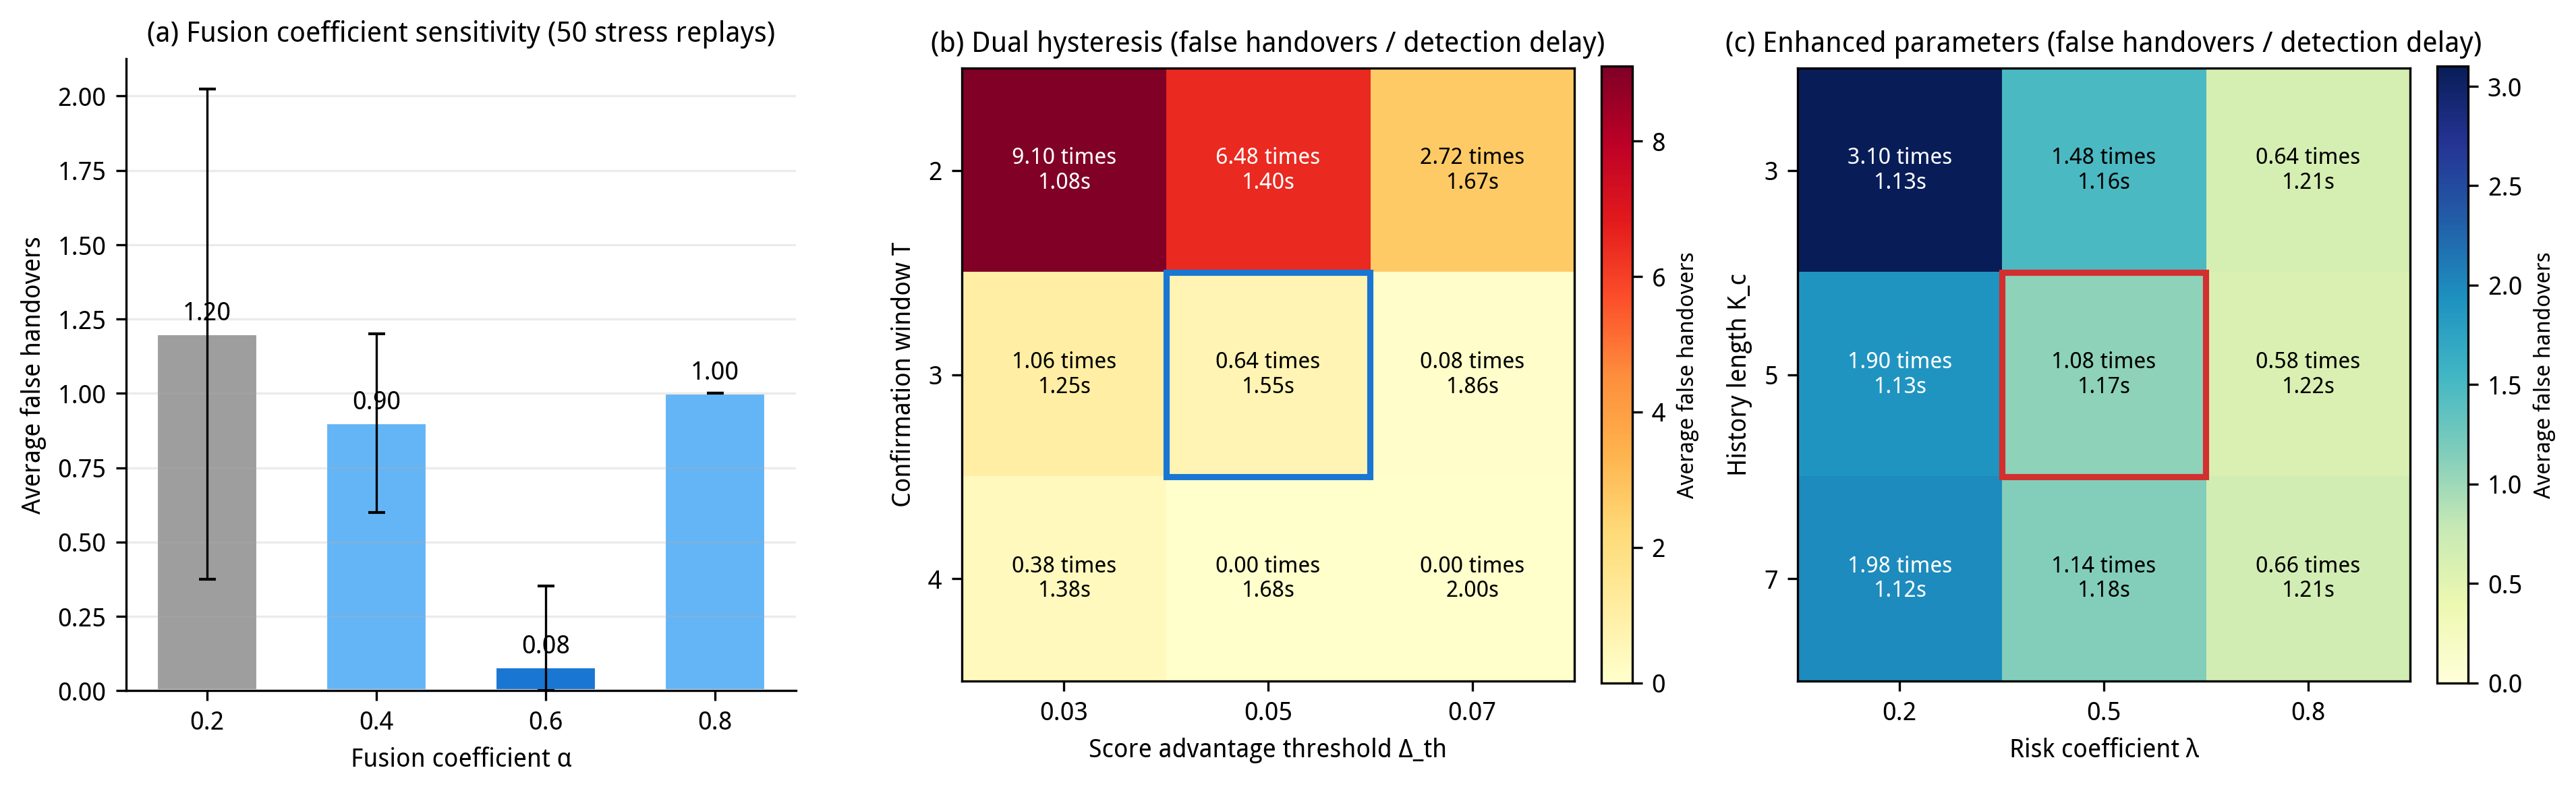
\includegraphics[width=\textwidth]{Figures/fig_parameter_sensitivity_en.png}
\caption{Sensitivity analysis of the fusion coefficient, dual-hysteresis parameters, and enhancement parameters. (For (\textbf{b}) and (\textbf{c}), upper entries denote mean false-handover counts and lower entries denote mean detection~delays.)}
\label{fig:param_sensitivity}
\end{figure}

Based on these parameter-selection experiments, Table~\ref{tab:params} summarizes the platform, network scenario, model architecture, and training/inference parameters. All comparison algorithms use the same simulation configuration, indicator sources, and analysis setting to avoid confounding algorithmic and environmental effects.

\begin{table}[H]
\centering
\caption{Experimental parameter settings.}
\small
\begin{tabularx}{\textwidth}{>{\raggedright\arraybackslash}p{4.6cm}>{\raggedright\arraybackslash}X}
\toprule
\textbf{Parameter} & \textbf{Value} \\
\midrule
Simulation platform & ns-3.45, ns3-ai, Python/PyTorch \\
Candidate networks & 5G, LTE, Wi-Fi \\
Algorithm scope & LAAVHA, 8 comparison algorithms, and 2 ablation variants \\
Runs & 250 trajectories (11-algorithm comparison); 50 (ablation/QoS) \\
Simulation duration & $50~\mathrm{s}$ per trajectory \\
Decision period & $0.1~\mathrm{s}$ \\
Decisions per run & 500 \\
Random seeds & 200--449 (11-algorithm comparison); 200--249 (ablation/QoS)\\
FlowMonitor mode & feed \\
Indicator dimensions & SINR, RSRP, delay, throughput, packet loss ratio \\
Position perturbation & $30~\mathrm{m}$ \\
Altitude perturbation & $10~\mathrm{m}$ \\
Time window $T_s$ & 10 \\
LSTM hidden units & 128 in the first layer, 64 in the second layer \\
Attention heads (num\_heads) & 1 (embed\_dim=5; single-head attention) \\
Fusion coefficient $\alpha$ & 0.6 \\
Dual-hysteresis parameters & $\Delta_{\mathrm{th}}=0.05$, confirmation window $T_h=3$ \\
Enhancement parameters & RS-TOPSIS closeness-history length $K_c=5$, RS-TOPSIS risk coefficient $\lambda=0.5$ \\
Training dataset & 10{,}000 samples (historical states and next-period targets) \\
Dataset split & training/validation = 80\%/20\% (sample-level random split; see text) \\
Loss function & MSE (mean squared error) for LSTM prediction only \\
Optimizer & Adam (learning rate = 0.001) \\
Batch size & 64 \\
Training epochs & 50 (maximum) \\
Early stopping & validation loss does not decrease for 10 consecutive epochs \\
Trainable parameters & LSTM layers ($\theta_1$, $\theta_2$) and prediction head ($W_{\mathrm{pred}}$, $b_{\mathrm{pred}}$) \\
Fixed parameters & Attention mechanism, $W_{\mathrm{mob}}$, and $W_{\mathrm{weight}}$ (Xavier uniform initialization) \\
\bottomrule
\end{tabularx}
\label{tab:params}
\end{table}

In addition to LAAVHA, the experiments evaluate eight comparison algorithms, namely TOPSIS-Q, Fuzzy-VHO, SAW, VIKOR, GRA, COPRAS, SPOTIS, and strongest-signal selection, plus the ablation variants LAAVHA-L and LAAVHA-A. These methods represent seven decision paradigms: fuzzy logic (Fuzzy-VHO), SAW, compromise ranking (VIKOR), distance-based ranking (TOPSIS-Q), relational analysis (GRA), proportional assessment (COPRAS), and reference-point ranking (SPOTIS). TOPSIS-Q follows TOPSIS network selection with entropy-weighted improved TOPSIS \cite{ref8,ref9,ref10}; Fuzzy-VHO follows fuzzy handover for 5G UAV networks \cite{ref4}; VIKOR uses compromise ranking \cite{ref11}; and GRA, COPRAS, SPOTIS, and SAW represent mainstream multi-attribute mobility decision methods \cite{ref12}. Strongest-signal selection chooses the candidate with the highest SINR. LAAVHA-L removes LSTM prediction, replacing predicted states with current states while retaining attention weights and dual hysteresis. LAAVHA-A removes attention-based dynamic weighting, retaining LSTM prediction and dual hysteresis while using entropy weighting for TOPSIS.

The LSTM prediction module requires training before deployment. To ensure valid generalization evaluation, the training and testing datasets must use disjoint random seeds. The training dataset uses seeds 0--199 to generate 10,000 supervised samples (historical 10-step windows paired with next-period ground-truth states). Seeds 200--449 are reserved exclusively for testing: all 250 seeds (200--449) are used for the 11-algorithm handover-count comparison and ablation study, while the first 50 of these (200--249) are additionally used for QoS evaluation. This separation prevents temporal information leakage and ensures that all performance metrics reflect the model's ability to generalize to unseen trajectories rather than memorize training scenarios.

As described above, the training dataset contains 10,000 samples collected from seeds 0--199. Each sample is a pre-built 10-step history window drawn from a distinct simulation episode; adjacent samples in the dataset originate from different runs rather than consecutive time steps of the same trajectory. Samples are therefore statistically independent, and the 80\%/20\% split in Table~\ref{tab:params} is applied at the sample level with no risk of temporal information leakage between training and validation subsets. Min-max normalization is performed per decision period within the simulation at inference time, scaling each of the five indicators across the three candidate networks to $[0,1]$; the normalization bounds are derived solely from the three-candidate values at that instant and are not fitted or shared across the dataset.

A handover event denotes a change in the network identifier selected by LAAVHA, rather than an actual Wi-Fi disassociation, LTE detachment, or 5G new-radio protocol-stack handover. The 5G candidate uses a proxy link, with SINR and RSRP calculated by a position-based propagation model following wireless-propagation and link-budget principles \cite{ref34}. Transport indicators are obtained from FlowMonitor statistics for point-to-point proxy flows. Table~\ref{tab:metrics} summarizes the indicator sources for each candidate network.

\begin{table}[H]
\centering
\caption{Candidate-network indicator sources.}
\small
\begin{tabularx}{\textwidth}{>{\raggedright\arraybackslash}p{1.3cm}>{\raggedright\arraybackslash}X>{\raggedright\arraybackslash}X>{\raggedright\arraybackslash}X>{\raggedright\arraybackslash}X}
\toprule
\textbf{Network} & \textbf{SINR/RSRP} & \textbf{Delay} & \textbf{Throughput} & \textbf{Packet loss ratio} \\
\midrule
Wi-Fi & Propagation proxy from MobilityModel position & FlowMonitor & PacketSink bytes received within interval & FlowMonitor \\
LTE & Propagation proxy from MobilityModel position & FlowMonitor & FlowMonitor & FlowMonitor \\
5G & Propagation proxy to assumed gNB & Point-to-point proxy-flow FlowMonitor & Point-to-point proxy-flow FlowMonitor & Point-to-point proxy-flow FlowMonitor \\
\bottomrule
\end{tabularx}
\label{tab:metrics}
\end{table}

Table~\ref{tab:metrics} summarizes the sources of the five network-state indicators in Section~\ref{sec:sim}. SINR and RSRP represent physical-layer link quality and are derived from UAV-access-point/base-station positions using the propagation proxy model. Delay, throughput, and packet loss ratio mainly represent transport-layer service quality. Wi-Fi throughput is calculated from PacketSink bytes received between adjacent periods, whereas LTE and 5G transport indicators are obtained from FlowMonitor. The table defines indicator sources for the decision-level simulation platform rather than a complete real-network protocol-stack measurement procedure. All candidates provide identically dimensioned indicators within each decision period, which LAAVHA and comparison methods uniformly normalize before multi-attribute decision making, ensuring identical candidate states and avoiding collection-related bias.

\subsection{Horizontal Comparison of Algorithms}\label{sec:hcomp}

The results evaluate the two challenges at two levels. First, an 11-algorithm comparison, representative decision-process comparison, and ablation study assess whether LSTM prediction, attention-based dynamic weighting, and dual hysteresis improve candidate selection and handover stability. Second, scenario-adaptation experiments under sustained link degradation and abrupt channel changes, such as high-speed coverage-boundary crossings, assess whether ALERA's ADH and RS-TOPSIS preserve necessary handovers while suppressing false and ping-pong handovers. All experiments use the defined performance indicators without introducing additional unmeasured metrics.

To evaluate LAAVHA across decision paradigms, eight representative algorithms were tested under identical conditions. Fuzzy-VHO uses a Mamdani fuzzy-inference system to fuzzify SINR and RSRP and make rule-based decisions. SAW applies fixed weights and sums normalized attributes, representing the basic MADM approach. TOPSIS-Q uses entropy weighting and standard TOPSIS ranking without temporal prediction. GRA ranks candidates by grey relational grades relative to an ideal reference sequence and handles uncertain information. VIKOR balances group utility and individual regret. COPRAS separately evaluates benefit and cost criteria to derive overall utility. SPOTIS ranks candidates by distance to a reference point. Strongest-signal selection chooses the candidate with the highest SINR as a single-factor baseline. Figure~\ref{fig:ho_comparison} compares all 11 algorithms.

\begin{figure}[H]
\centering
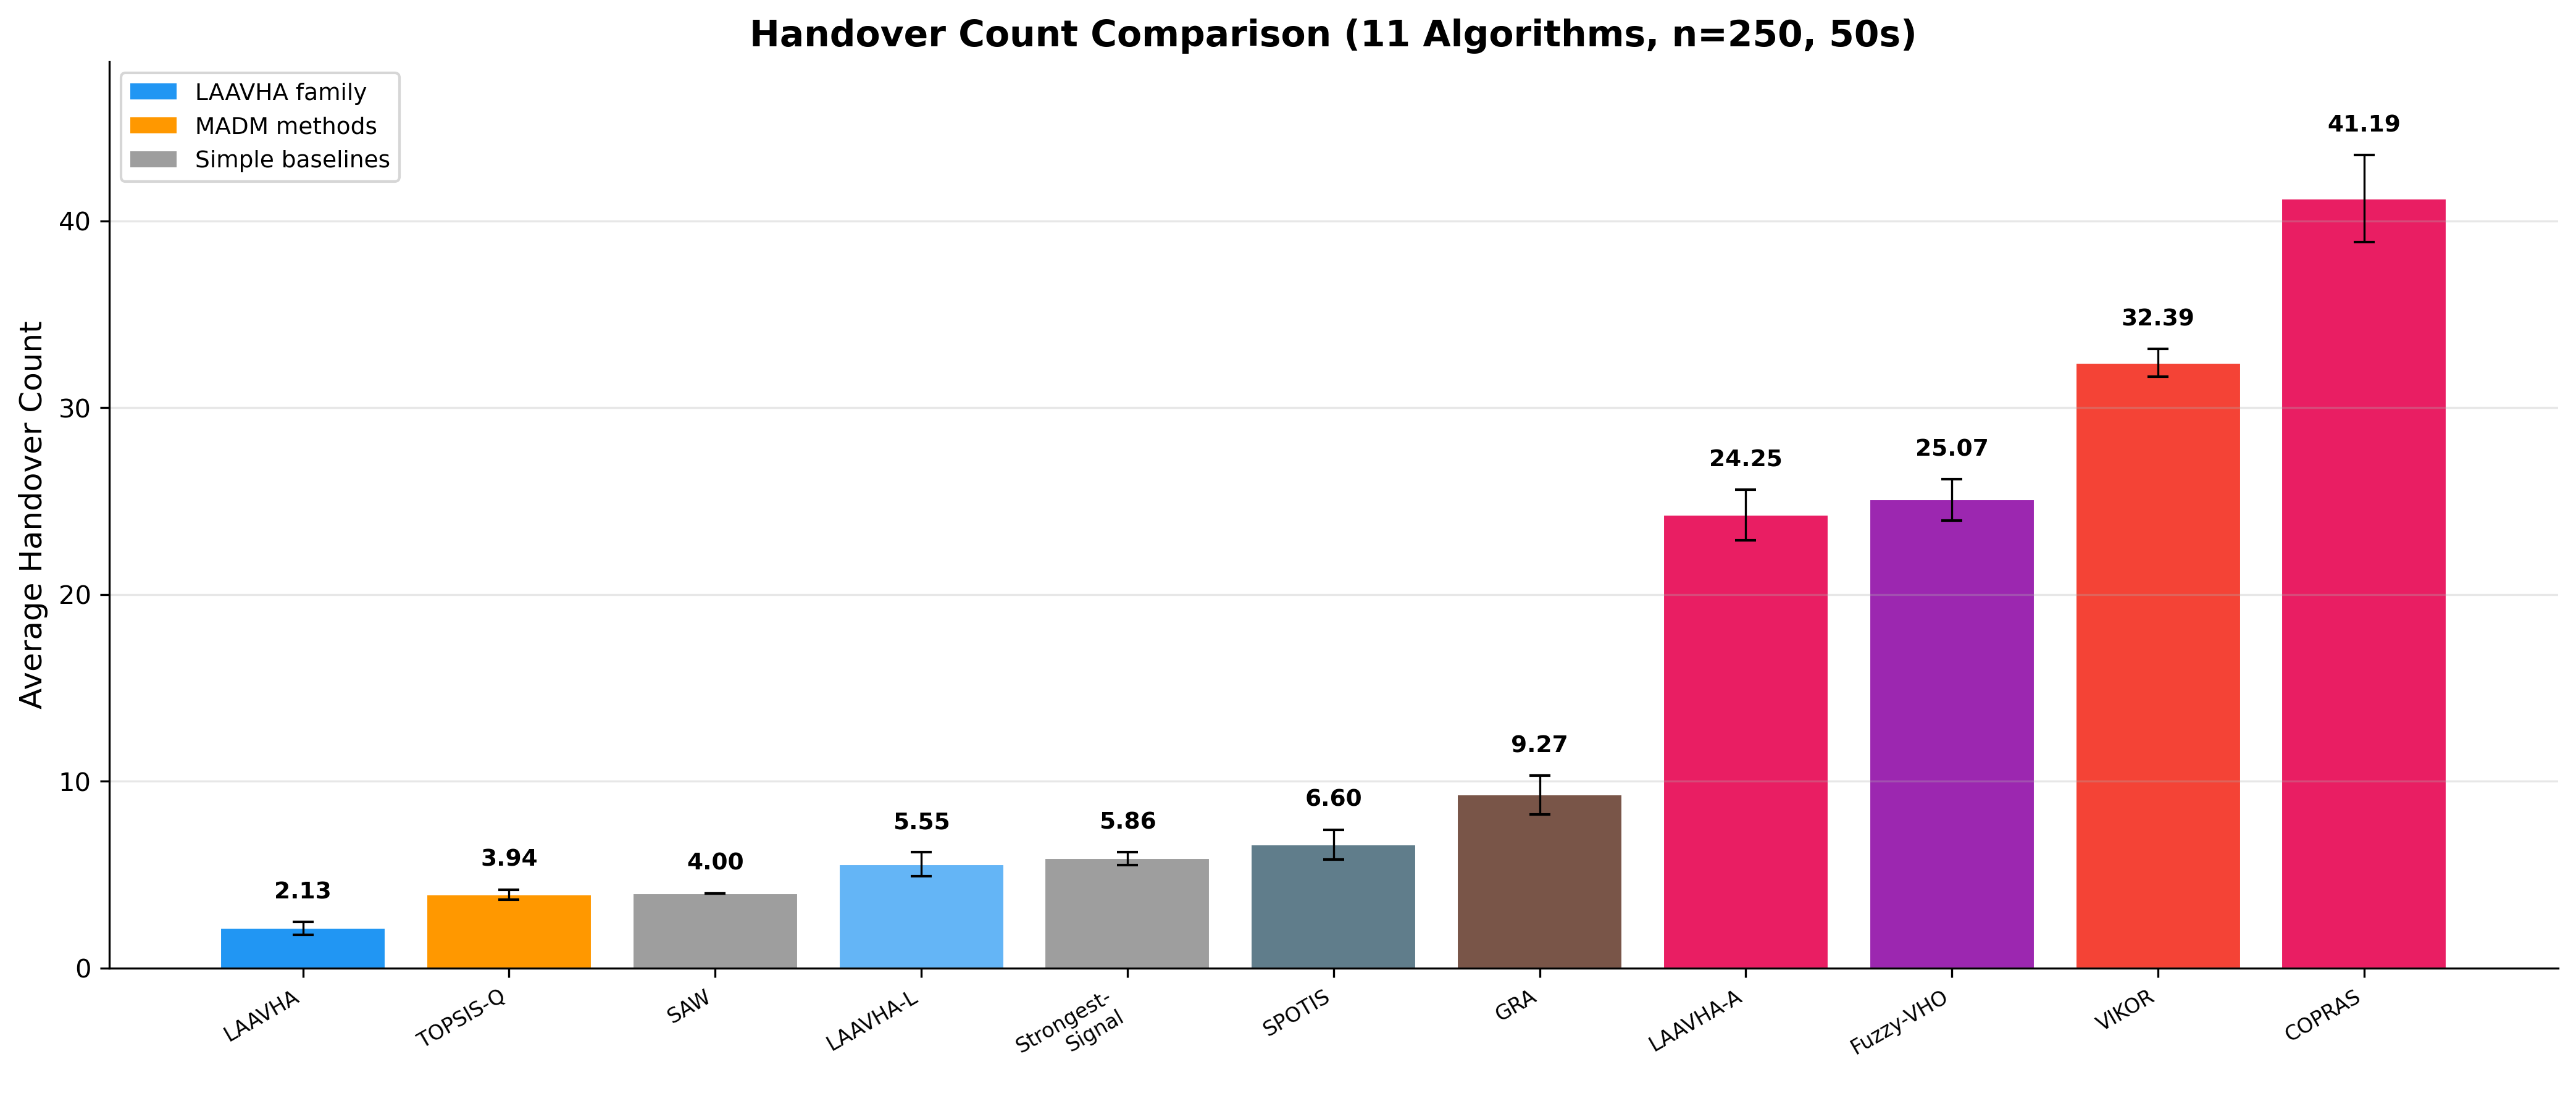
\includegraphics[width=\textwidth]{Figures/fig_handover_count_by_algorithm.png}
\caption{Mean handover-count comparison of 11 algorithms (mean $\pm$ std, \textit{n}=250, 50-second trajectories).}
\label{fig:ho_comparison}
\end{figure}

LAAVHA achieves the lowest mean handover count among 11 algorithms, at $2.13$ (Figure~\ref{fig:ho_comparison}). The three LAAVHA variants (LAAVHA $2.13$, LAAVHAL $5.55$, LAAVHAA $24.25$) demonstrate the contributions of individual components, with the full algorithm outperforming ablated versions. Among the baseline algorithms, TOPSIS-Q yields $3.94$, SAW $4.00$, strongest-signal selection $5.86$, SPOTIS $6.60$, GRA $9.27$, Fuzzy-VHO $25.07$, VIKOR $32.39$, and COPRAS $41.19$. MADM methods without temporal prediction (TOPSIS-Q, SAW, VIKOR, GRA, SPOTIS, COPRAS) exhibit elevated handover counts because fixed weights and instantaneous indicators cause repeated reassignments when candidate scores alternate near coverage boundaries. Strongest-signal selection considers only SINR, excluding delay, throughput, and packet loss. Fuzzy-VHO's rule-based membership functions respond reactively to local SINR and RSRP fluctuations. Overall, LAAVHA reduces handovers by $46.0\%-94.8\%$ versus the eight baselines, confirming that LSTM prediction and attention-based dynamic weighting suppress unnecessary reassignments in extended 50-second missions.

To address whether the low handover count reflects excessive conservatism, Table~\ref{tab:qos_comparison} and Figure~\ref{fig:qos_comparison} compare end-to-end communication quality across five representative algorithms under 50 extended-duration (50-second) scenarios (seeds 200--249). Three metrics are evaluated: mean throughput (Mbps), mean delay (ms), and mean packet loss ratio (\%). The results demonstrate that LAAVHA achieves the best or near-best performance in all three dimensions while maintaining the lowest handover frequency, refuting the hypothesis that reduced handovers necessarily compromise service quality.

\begin{table}[H]
\centering
\caption{End-to-end QoS comparison across five representative algorithms (mean $\pm$ std, \textit{n}=50, 50-second trajectories).}
\label{tab:qos_comparison}
\begin{tabular}{lccc}
\toprule
\textbf{Algorithm} & \textbf{Throughput (Mbps)} & \textbf{Delay (ms)} & \textbf{Packet Loss (\%)} \\
\midrule
LAAVHA          & $2.00 \pm 0.12$ & $1.00 \pm 0.15$ & $1.63 \pm 0.18$ \\
TOPSIS-Q        & $1.98 \pm 0.14$ & $1.06 \pm 0.18$ & $1.63 \pm 0.18$ \\
GRA             & $1.51 \pm 0.22$ & $1.39 \pm 0.26$ & $1.76 \pm 0.24$ \\
Strongest-Signal & $0.24 \pm 0.08$ & $2.29 \pm 0.42$ & $1.57 \pm 0.20$ \\
VIKOR           & $1.78 \pm 0.18$ & $1.20 \pm 0.21$ & $1.62 \pm 0.20$ \\
\bottomrule
\end{tabular}
\end{table}

\begin{figure}[H]
\centering
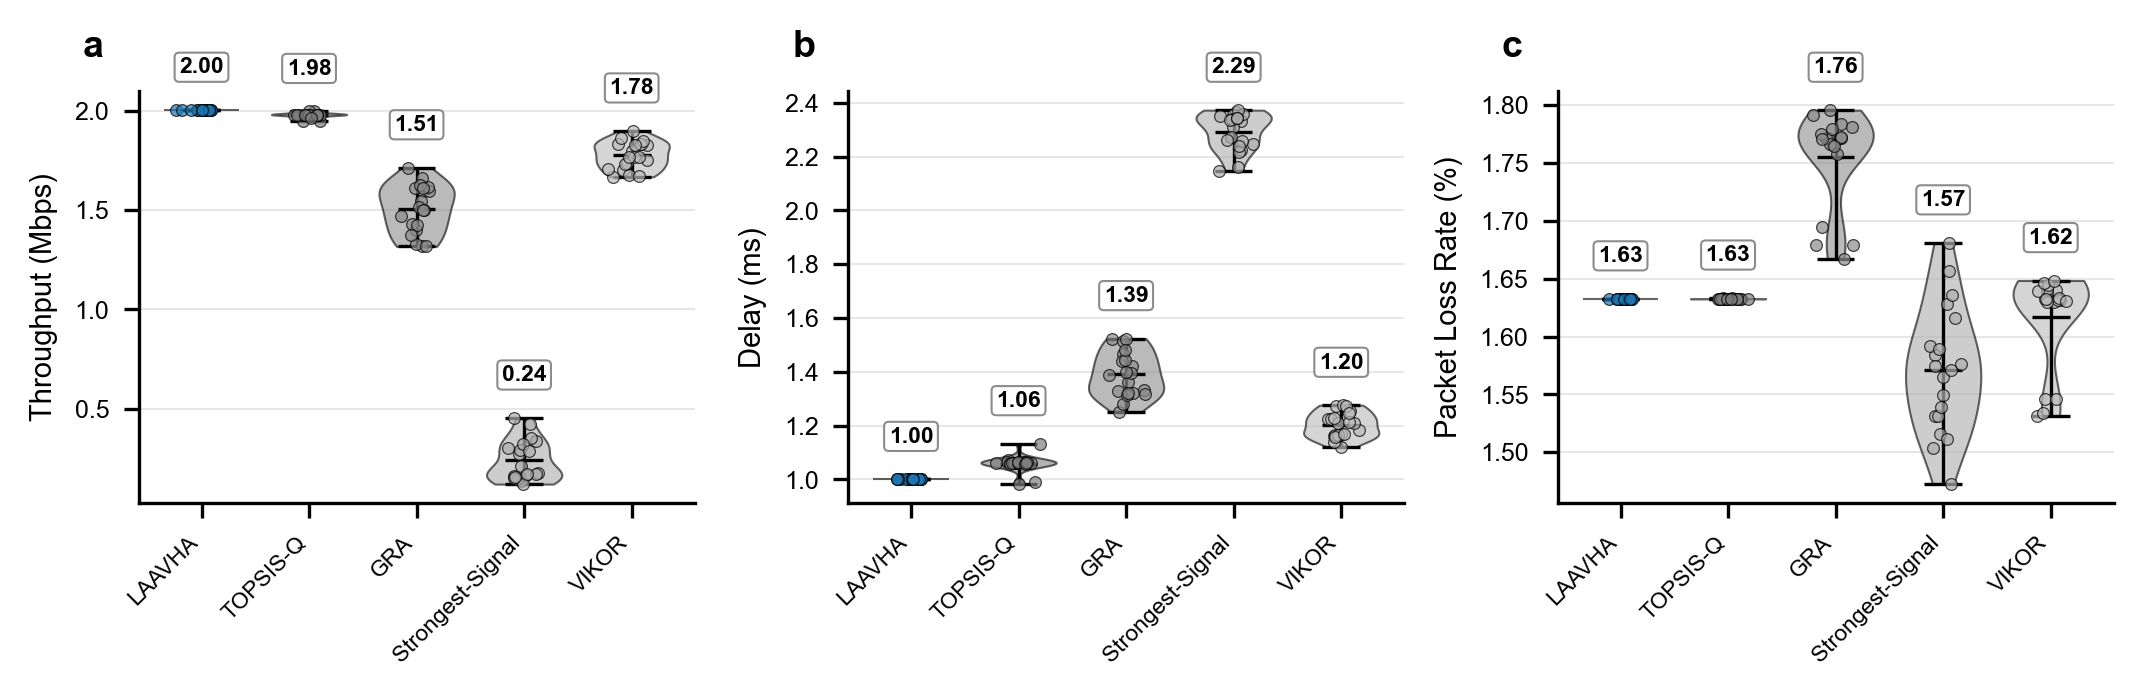
\includegraphics[width=\textwidth]{Figures/qos_comparison_nature.png}
\caption{QoS metric distributions across five representative algorithms (\textit{n}=50). (\textbf{a}) Throughput, (\textbf{b}) delay, (\textbf{c}) packet loss ratio. Violin plots show density; points denote individual runs, and horizontal bars mark the mean and range.}
\label{fig:qos_comparison}
\end{figure}

LAAVHA achieves the highest mean throughput ($2.00$ Mbps) and lowest mean delay ($1.00$ ms), while maintaining low packet loss ($1.63\%$), identical to TOPSIS-Q ($1.63\%$), below GRA ($1.76\%$), and slightly higher than strongest-signal selection ($1.57\%$) and VIKOR ($1.62\%$). Notably, strongest-signal selection---despite achieving the lowest packet loss---suffers severely degraded throughput ($0.24$ Mbps, an $88\%$ reduction) and elevated delay ($2.29$ ms, $129\%$ higher), demonstrating that optimizing a single metric does not guarantee overall service quality. LAAVHA's balanced performance across all three QoS dimensions confirms that handover reduction stems from intelligent multi-attribute decision-making rather than single-factor optimization. LSTM prediction and attention-based dynamic weighting enable stable network selection, choosing candidates capable of sustaining service throughout extended missions while minimizing unnecessary reassignments.

The QoS results further substantiate this interpretation. The low handover count reflects intelligent decision-making rather than excessive conservatism. LSTM prediction and attention-based dynamic weighting enable accurate candidate evaluation over extended 50-second trajectories, selecting networks capable of sustaining service throughout the mission while minimizing unnecessary reassignments. The dual-hysteresis mechanism ($\Delta_{\mathrm{th}}=0.05, T_h=3$) filters transient boundary fluctuations but does not prevent necessary handovers when sustained degradation occurs. When LAAVHA does trigger handovers, it responds to genuine network-state changes as conditions evolve across coverage boundaries, rather than reacting to transient signal variations. In contrast, baseline algorithms without temporal awareness trigger handovers reactively when current-state scores cross decision boundaries, producing unnecessary reassignments from transient signal variations near coverage edges. This distinction is validated by ALERA's behavior under forced degradation (Section~\ref{sec:adapt}), where the algorithm completes all necessary handovers in Zone 1 while suppressing false handovers in Zone 2, demonstrating that low handover frequency results from stable decision-making, not failure to act when conditions warrant reassignment.

\subsection{Comparison of Representative Decision Processes}\label{sec:process}

To validate the algorithm behaviors described in Section~\ref{sec:laavha}, a representative 50-second trajectory (seed=200) was selected from the 250-trajectory test set (seeds 200--449) that traverses the coverage boundaries defined in Figure~\ref{fig:network_coverage}. The UAV departs from a 5G-dominant region, crosses Wi-Fi hotspot edges near imaging sites, and enters LTE-covered areas, creating natural opportunities for vertical handover. This extended duration allows full observation of handover decision evolution across multiple network transitions, consistent with the 50-second trajectories used in the aggregate comparison experiments.

Figure~\ref{fig:scoring} compares LAAVHA, TOPSIS-Q, and Fuzzy-VHO under this scenario in a two-row, three-column layout. The selection emphasizes explanatory value rather than aggregate handover count. TOPSIS-Q shares LAAVHA's TOPSIS framework but lacks LSTM prediction, attention-based dynamic weighting, and dual hysteresis, providing a controlled comparison of their effects on closeness stability and handover triggering. Fuzzy-VHO represents a rule-based paradigm driven by fuzzy membership functions and rules, making it more sensitive to local SINR and RSRP fluctuations. Together, they assess dynamic multi-attribute fusion against rule-based handover. Although strongest-signal selection and SAW achieve lower mean counts, strongest-signal uses only SINR and SAW uses fixed weighted sums; neither provides a temporal decision process comparable to LAAVHA and is therefore more suitable for aggregate-statistic comparison.

The upper panels show the integrated TOPSIS closeness scores for 5G, LTE, and Wi-Fi, where values closer to 1 indicate better network service quality; the lower panels show their SINR (dB) under the same simulation, with red dashed lines marking handover times. As the UAV moves from 5G-dominant areas through Wi-Fi hotspot boundaries into LTE-covered regions, candidate SINR and closeness scores fluctuate naturally due to the heterogeneous coverage transitions designed in the simulation scenario (Figure~\ref{fig:network_coverage}). LAAVHA maintains relatively stable decisions with only 2 handovers over the 50-second trajectory, corresponding to the two necessary network transitions when the UAV crosses major coverage boundaries: from the initial 5G-dominant region into the Wi-Fi hotspot zone, and subsequently into the LTE-covered area. These handovers reflect intelligent adaptation to the coverage topology rather than algorithmic instability. Dual hysteresis ($\Delta_{\mathrm{th}}=0.05, T_h=3$) and temporal prediction suppress reactive reassignments caused by transient fluctuations within each coverage region. Although 5G does not always have the largest SINR, attention-based dynamic weights incorporate delay, throughput, packet loss ratio, and other attributes, maintaining its selection during most of the mission. In contrast, TOPSIS-Q triggers 6 handovers when 5G and Wi-Fi closeness scores converge repeatedly near coverage boundaries, while Fuzzy-VHO responds aggressively to SINR fluctuations with 13 handovers. These results demonstrate the stabilizing effects of temporal prediction and dynamic weighting.

\begin{figure}[H]
\centering
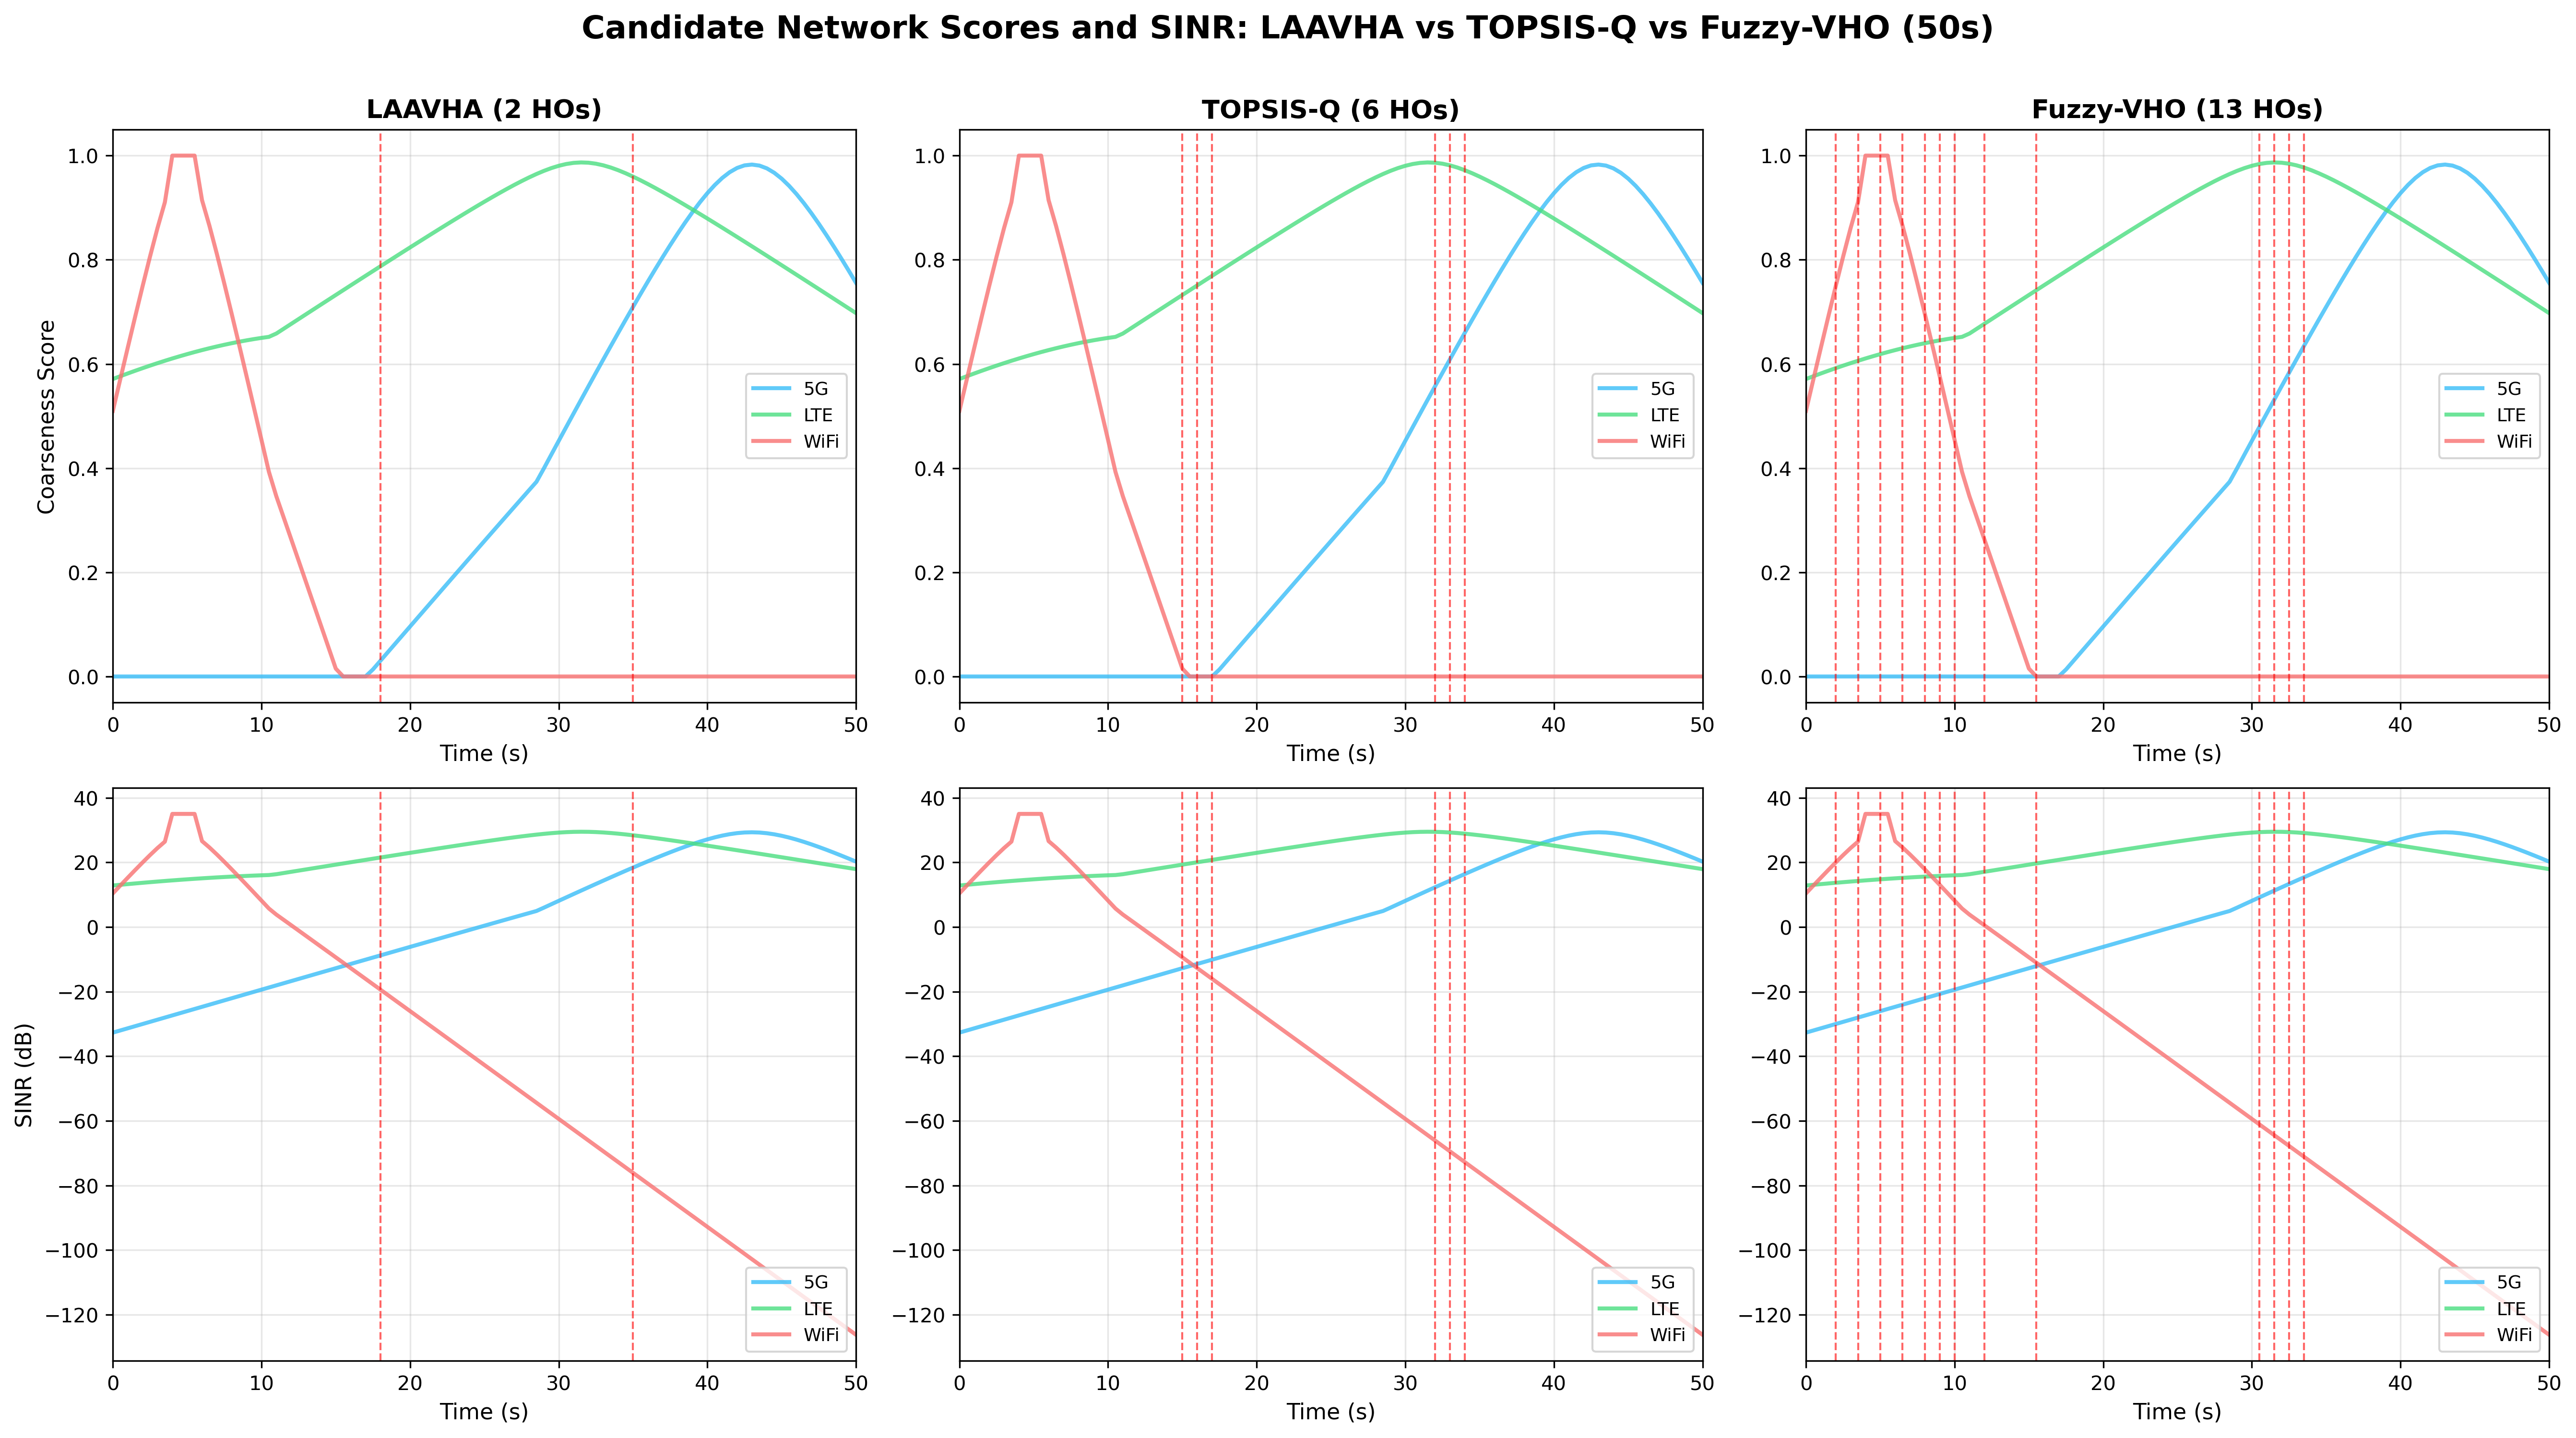
\includegraphics[width=\textwidth]{Figures/fig_scoring_timeline_comparison_50s_ideal.png}
\caption{Candidate-network scores and SINR time series for LAAVHA, TOPSIS-Q, Fuzzy-VHO under a 50-second representative trajectory (seed=200) traversing the coverage boundaries in Figure~\ref{fig:network_coverage}. Vertical lines indicate handovers.}
\label{fig:scoring}
\end{figure}

\subsection{Ablation-Study Validation}\label{sec:ablation}

Ablation experiments quantify the contributions of LSTM prediction and attention-based dynamic weighting to LAAVHA. LAAVHA-L removes LSTM prediction by setting the predicted state equal to the current state while retaining attention weighting, improved TOPSIS, and dual hysteresis, testing temporal prediction. LAAVHA-A removes attention-based dynamic weighting, retains LSTM prediction, improved TOPSIS, and dual hysteresis, and replaces attention weights with entropy weights, testing dynamic-weight learning. Both variants and full LAAVHA use the same 250 random seeds (200$-$449) and 50-second simulation parameters. Figure~\ref{fig:ablation} presents handover counts with scatter-overlaid bars, where each point represents one run, bar height is the mean, and error bars indicate $\pm1$ standard deviation. LAAVHA achieves 2.13 (std=0.34), demonstrating stable cooperation between prediction and dynamic weighting in extended trajectories. LAAVHA-L increases to 5.55 (std=0.64), showing that removing temporal prediction produces more reactive decisions and 160\% more handovers. LAAVHA-A reaches 24.25 (std=1.35), indicating that entropy weighting cannot adapt criteria to the flight phase and leads to frequent handovers. The full algorithm achieves an 11.4-fold reduction (2.13 vs. 24.25) compared to the no-attention variant, confirming that dynamic weight adaptation is essential for handover stability. Notably, this improvement is achieved despite the attention module having never been trained via gradient descent (Section~\ref{sec:weight}); its parameters were initialized using Xavier uniform and remained fixed throughout training. The result validates that the attention mechanism's structural design---query-key attribute interaction combined with mobility-aware projection---provides sufficient adaptivity through its architectural inductive bias alone, without requiring end-to-end optimization.

\begin{figure}[H]
\centering
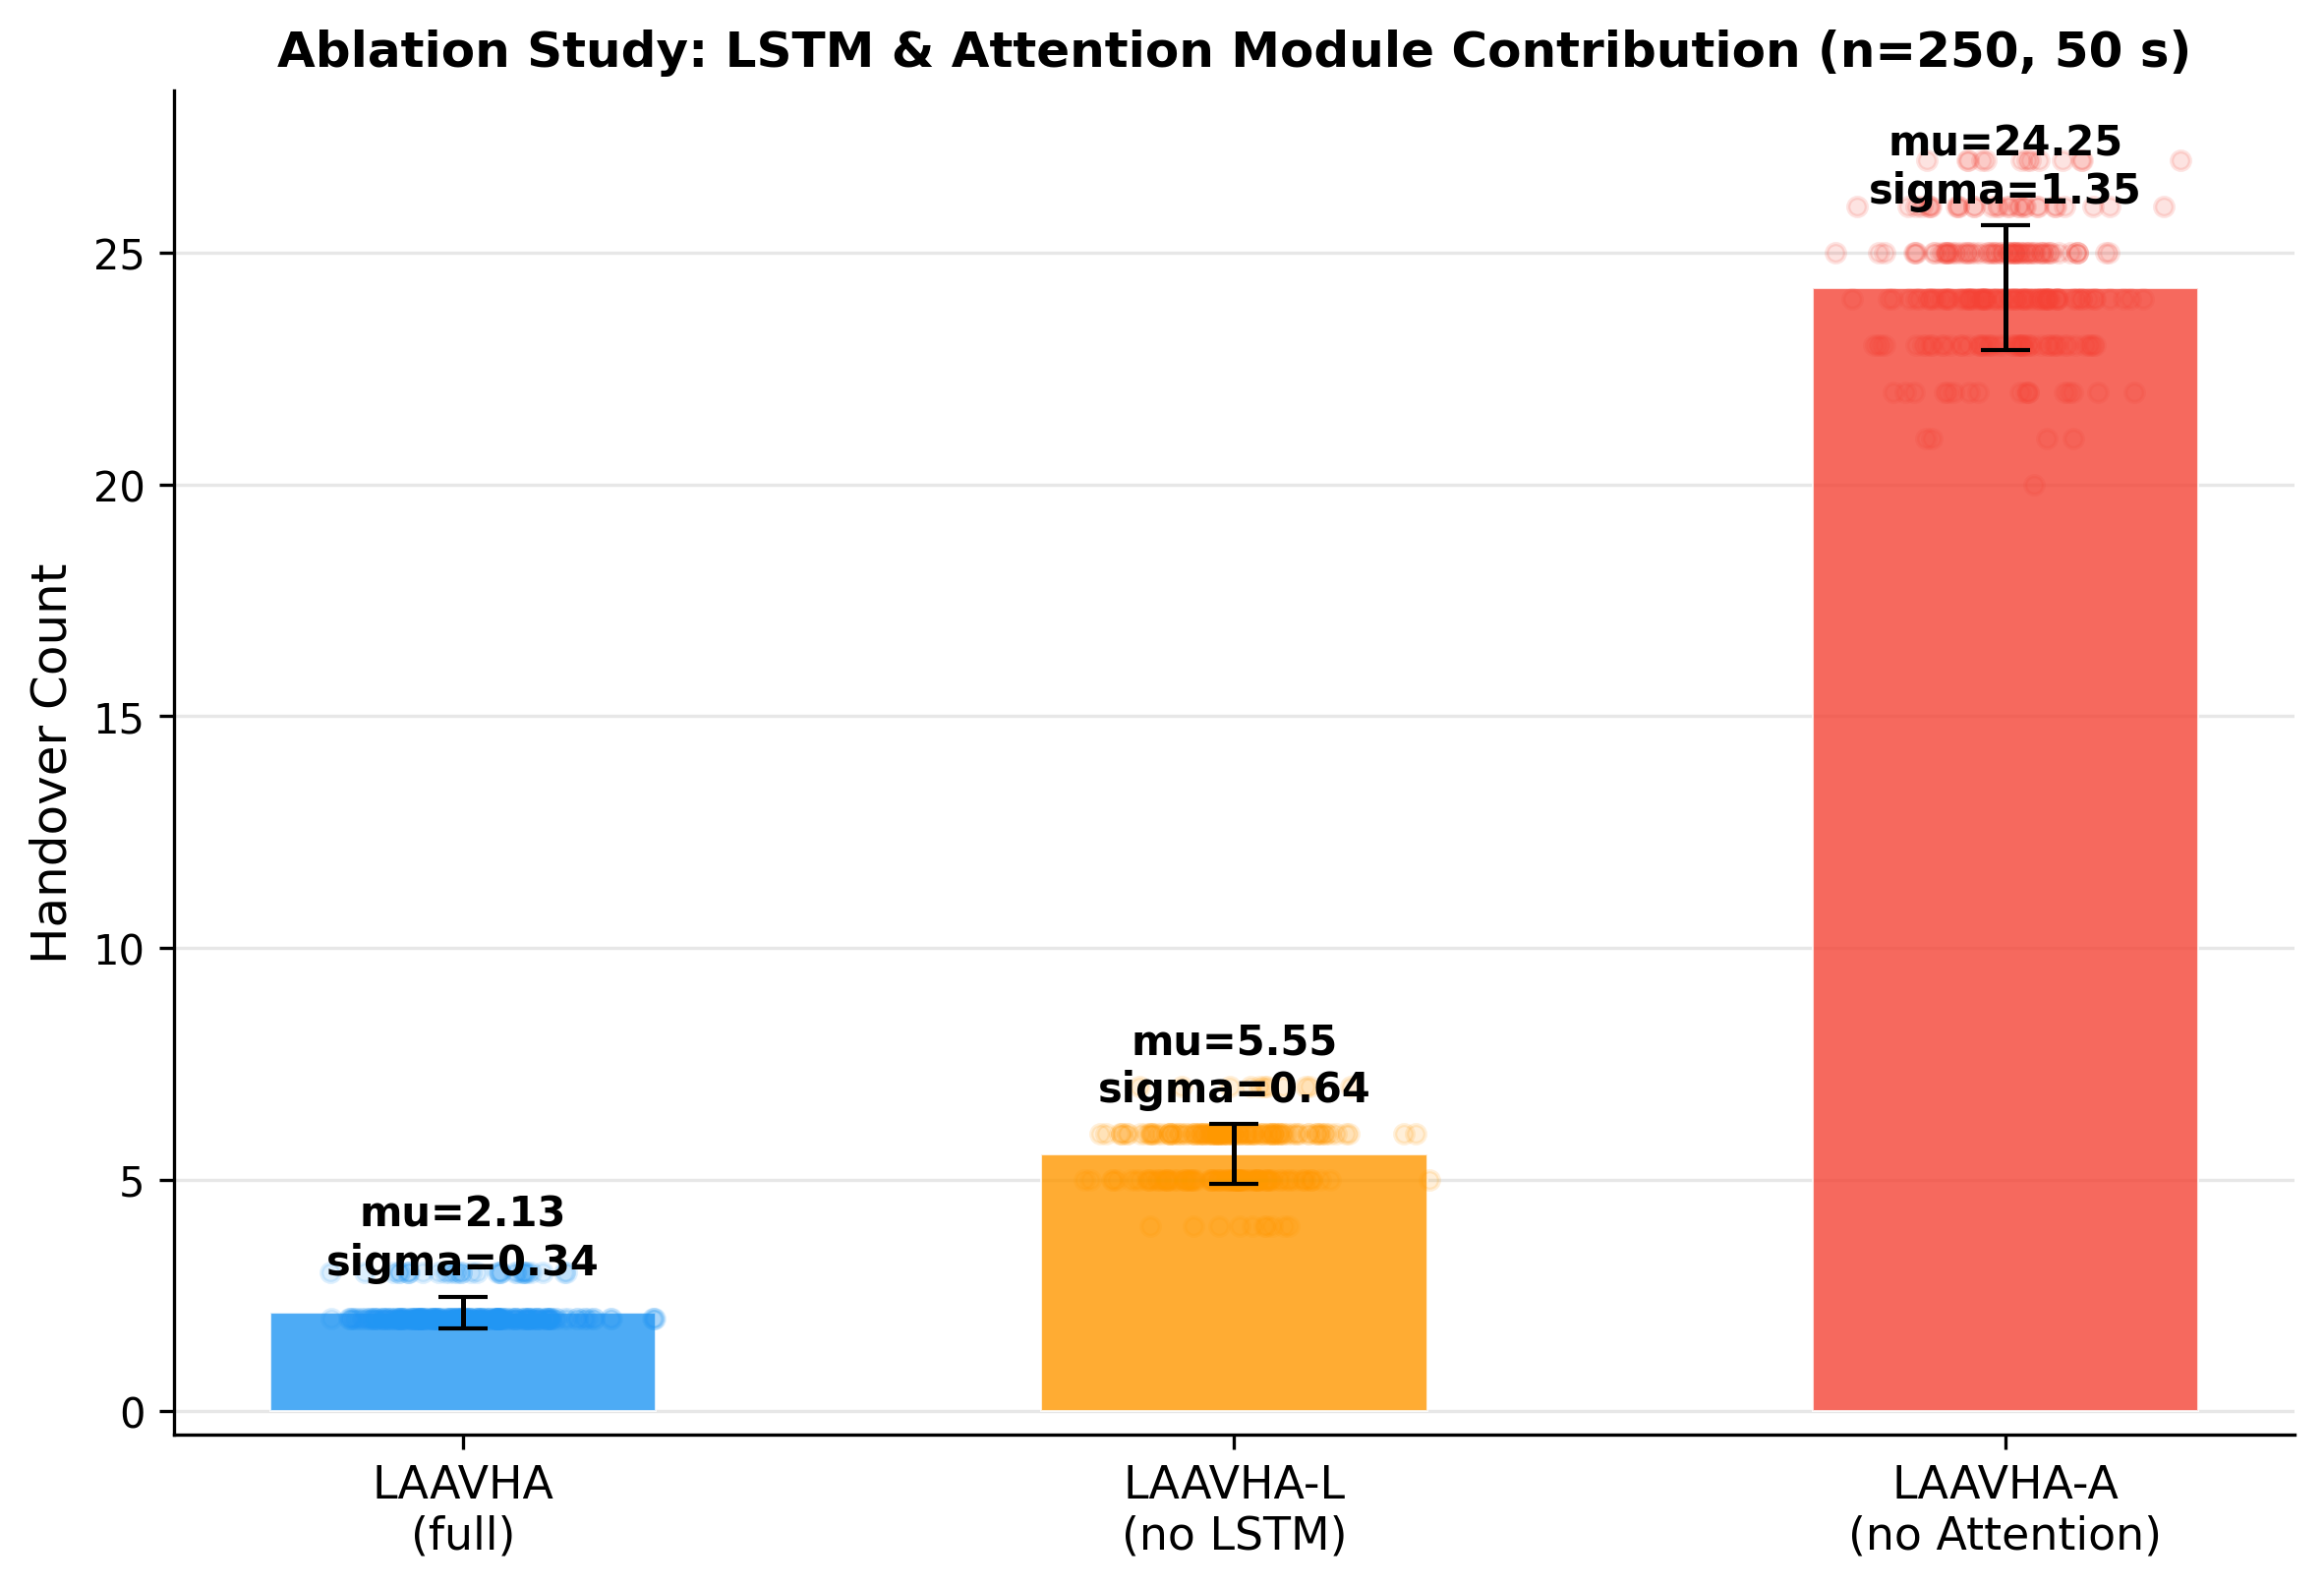
\includegraphics[width=0.68\textwidth]{Figures/fig_laavha_handover_count.png}
\caption{Handover-count comparison in the LAAVHA ablation study (mean $\pm$ std, \textit{n}=250, 50-second trajectories).}
\label{fig:ablation}
\end{figure}

The ablation results demonstrate strong synergy between LSTM prediction and attention-based dynamic weighting; neither module alone maintains low handover frequency in extended trajectories. Removing attention has the largest effect, increasing the mean from 2.13 to 24.25, an 11.4-fold rise, showing that flight- and network-state-based weights adapt to phase-specific requirements far better than static entropy weights. Removing the LSTM increases the mean to 5.55, confirming that temporal prediction contributes an additional 61\% reduction (5.55$\rightarrow$2.13) beyond dynamic weighting alone. Together, these results validate the LAAVHA architecture: LSTM prediction provides temporal smoothing, while attention-based weighting prevents the ping-pong effect caused by fixed weights near coverage boundaries.

\subsection{Scenario Adaptation and Enhancement Validation}\label{sec:adapt}

To evaluate ALERA under rapid coverage-boundary crossings and abrupt channel changes, a competitive scenario is constructed with network A, analogous to 5G, and network B, analogous to Wi-Fi, having closeness scores near 0.50; A is initially serving. The scenario represents two data transmission conditions: timely migration under sustained degradation and handover suppression under transient disturbances from short obstructions or multipath effects. Figure~\ref{fig:enhanced} shares the time axis across four panels, with $t=5-8~\mathrm{s}$ and $t=12-15~\mathrm{s}$ denoting the same intervals in panels a--d. Light-blue Zone 1 represents sustained degradation, where A declines and B improves, requiring a correct A-to-B handover. Light-red Zone 2 represents transient fluctuations, where sinusoidal variation and Gaussian noise are injected into B; short peaks provide no sustained mean advantage and should not trigger handover.

Panel (a) of Figure~\ref{fig:enhanced} shows raw closeness curves. The vertical axis represents the candidate's integrated score before risk penalization, with higher values indicating greater proximity to the ideal candidate. Network B maintains a persistent advantage in Zone 1, whereas its Zone 2 increase is a transient high-frequency oscillation.

Panel (b) shows handovers under the fixed low threshold ($\Delta_{\mathrm{th}}=0.03$); the vertical axis is raw closeness, and red dashed lines mark handover times and directions. Correct A$\rightarrow$B and B$\rightarrow$A handovers occur at $t=6.6~\mathrm{s}$ and $t=11.9~\mathrm{s}$, respectively, corresponding to sustained degradation and subsequent recovery. In Zone 2, transient peaks trigger A$\rightarrow$B at $t=14.8~\mathrm{s}$ and B$\rightarrow$A at $t=15.1~\mathrm{s}$, producing a false handover and subsequent ping-pong handover.

Panel (c) presents ALERA's risk-adjusted scores, with the vertical axis $C_i^{\mathrm{robust}}=C_i-\lambda\sigma_i^C$, with green dashed lines indicating handovers. ALERA retains both necessary handovers while suppressing Zone 2 fluctuations and avoiding handover.

Panel (d) shows the adaptive threshold $\Delta_{\mathrm{th}}$, representing the required closeness advantage. In Zone 2, it increases from 0.03 to approximately 0.08 and gradually decreases after fluctuations subside, demonstrating that ADH raises the handover barrier only under unstable conditions.

The enhancement provides two key benefits. Under sustained degradation, it completes the necessary handover from degraded network A to better network B, avoiding excessive conservatism. Under transient variation, it suppresses false handovers caused by short peaks and prevents A$\rightarrow$B$\rightarrow$A ping-pong. RS-TOPSIS reduces the ranking advantage of volatile candidates, determining which network to switch to, while ADH raises the trigger threshold during fluctuations, determining when to switch. Together, they preserve necessary handovers, reduce false handovers, and limit associated link-reestablishment overhead.

\begin{figure}[H]
\centering
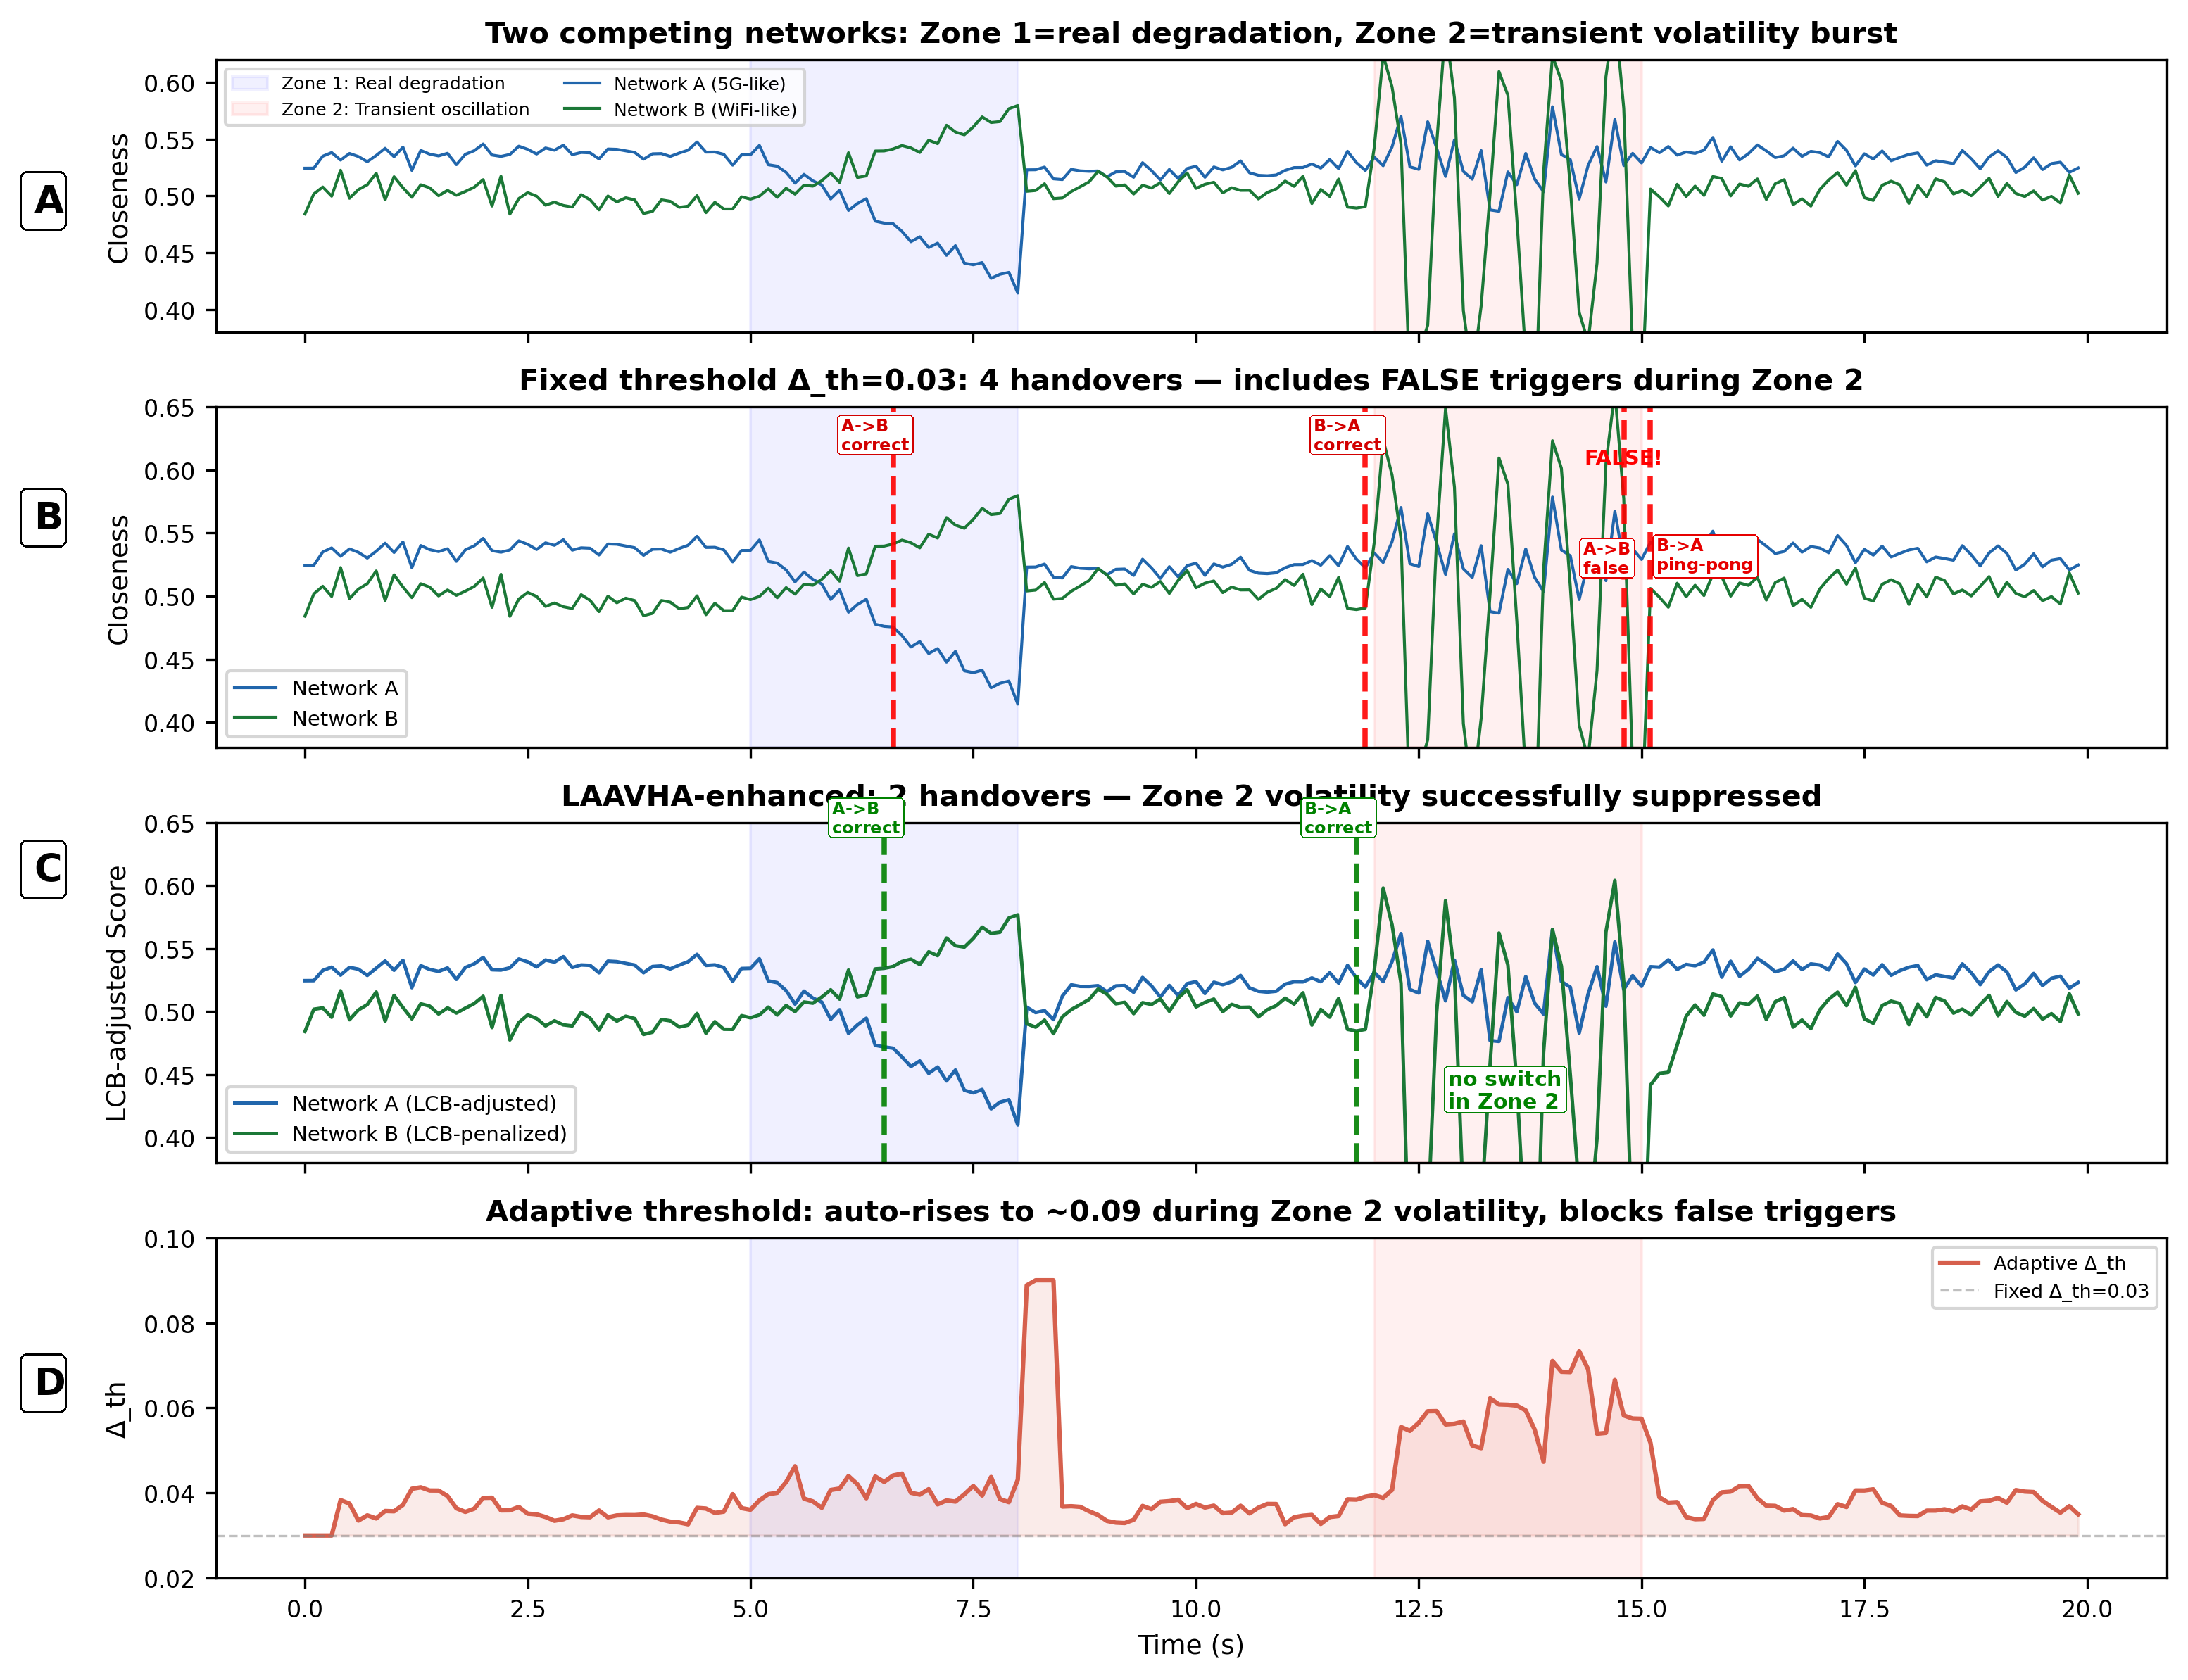
\includegraphics[width=0.86\textwidth]{Figures/fig_adaptive_hysteresis_proof.png}
\caption{Adaptive-hysteresis validation of fixed low threshold ($\Delta_{\mathrm{th}}=0.03$) and ALERA under sustained degradation and transient fluctuation.}
\label{fig:enhanced}
\end{figure}

\section{Conclusion}\label{sec:conclusion}

For VHO challenges arising from wide-area flight, heterogeneous coverage, and rapid link-state changes in UAV heterogeneous wireless networks, this paper proposes LAAVHA and its enhanced version, ALERA. LAAVHA integrates stacked-LSTM short-term state prediction, attention-based dynamic attribute weighting, improved TOPSIS using current and predicted states, and dual-hysteresis decision-making. This joint use of temporal evolution, flight state, and multi-attribute service requirements reduces handovers caused by transient boundary fluctuations. Without altering the LSTM-attention architecture or training parameters, ALERA adds ADH to adapt the handover threshold and confirmation window to serving-network SINR variation and flight speed, and RS-TOPSIS to penalize historical closeness variation. Therefore, it improves adaptation through both ``when to switch'' and ``which network to switch to.'' Across 250 extended 50-second trajectories, LAAVHA achieves the lowest mean decision-level handover count among 11 algorithms ($2.13$), reducing handovers by $46.0\%-94.8\%$ versus eight baselines while maintaining the highest throughput and lowest delay among evaluated algorithms. Removing LSTM prediction or dynamic attention weighting increases the mean to $5.55$ and $24.25$, respectively, confirming their complementary roles in handover stability. At the decision level, ALERA completes all necessary network selection changes under sustained degradation and produces zero false changes under transient variation, demonstrating stable decision-making for UAV aerial missions in heterogeneous wireless networks.

%=================================================================
%% References
\begin{thebibliography}{999}
\bibitem{ref1}
Yang, K.; Wang, Y.; Gao, X.; et al. Communications in space--air--ground integrated networks: An overview. {\em Space Sci. Technol.} 2025, 5, 0199.
\bibitem{ref2}
Geraci, G.; García-Rodríguez, A.; Azari, M.M.; et al. What will the future of UAV cellular communications be? A flight from 5G to 6G. {\em IEEE Commun. Surv. Tutor.} 2022, 24, 1304--1335. DOI: 10.1109/COMST.2022.3171135.
\bibitem{ref3}
Ribeiro, L.M.B.; Müller, I.; Becker, L.B. Communication interface manager for improving performance of heterogeneous UAV networks. {\em Sensors} 2021, 21, 4255.
\bibitem{ref4}
Ayass, T.; Coqueiro, T.; Carvalho, T.; et al. Unmanned aerial vehicle with handover management fuzzy system for 5G networks: Challenges and perspectives. {\em Intell. Robot.} 2022, 2, 20--36.
\bibitem{ref5}
Rehman, A.U.; Roslee, M.B.; Tiang, J.J. A survey of handover management in mobile HetNets: Current challenges and future directions. {\em Appl. Sci.} 2023, 13, 3367.
\bibitem{ref6}
Haghrah, A.; Abdollahi, M.P.; Azarhava, H.; et al. A survey on the handover management in 5G-NR cellular networks: Aspects, approaches and challenges. {\em EURASIP J. Wirel. Commun. Netw.} 2023, 2023, 52.
\bibitem{ref7}
Wang, Z.; Lv, Z.; Xu, X.; et al. Vertical switching algorithm for unmanned aerial vehicle in power grid heterogeneous communication networks. {\em Electronics} 2024, 13, 2612.
\bibitem{ref8}
Zhong, J.; Zhang, L.; Alhabo, M.; et al. A hybrid scheme using TOPSIS and Q-learning for handover decision making in UAV-assisted heterogeneous network. {\em IEEE Access} 2024, 12, 31422--31430. DOI: 10.1109/ACCESS.2024.3368916.
\bibitem{ref9}
Goh, M.I.; Mbulwa, A.I.; Yew, H.T.; et al. Handover decision-making algorithm for 5G heterogeneous networks. {\em Electronics} 2023, 12, 2384.
\bibitem{ref10}
Hwang, C.L.; Yoon, K. \textit{Multiple Attribute Decision Making: Methods and Applications. A State-of-the-Art Survey}; Springer-Verlag: Berlin, Germany, 1981.
\bibitem{ref11}
Zolfani, S.; Yazdani, M.; Pamucar, D.; et al. A VIKOR and TOPSIS focused reanalysis of the MADM methods based on logarithmic normalization. {\em Facta Univ. Ser. Mech. Eng.} 2020, 18, 341--355.
\bibitem{ref12}
Dantas Silva, F.S.; Lima, M.P.S.; Corujo, D.; et al. A comprehensive step-wise survey of multiple attribute decision-making mobility approaches. {\em IEEE Access} 2024, 12, 108616--108656. DOI: 10.1109/ACCESS.2024.3436074.
\bibitem{ref13}
Satapathy, P.; Mahapatro, J. An efficient multicriteria-based vertical handover decision-making algorithm for heterogeneous networks. {\em Trans. Emerg. Telecommun. Technol.} 2022, 33, e4409.
\bibitem{ref14}
Zhong, Y.; Wang, H.; Lv, H.; et al. A vertical handover decision scheme using subjective-objective weighting and grey relational analysis in cognitive heterogeneous networks. {\em Ad Hoc Netw.} 2022, 134, 102924.
\bibitem{ref15}
Riaz, H.; Öztürk, S.; Aldirmaz Çolak, S.; et al. Performance analysis of weighting methods for handover decision in HetNets. {\em Gazi Univ. J. Sci.} 2024, 37, 1791--1810.
\bibitem{ref16}
Tan, K.; Bremner, D.; Le Kernec, J.; et al. Intelligent handover algorithm for vehicle-to-network communications with double-deep Q-learning. {\em IEEE Trans. Veh. Technol.} 2022, 71, 7848--7862.
\bibitem{ref17}
Jang, Y.; Raza, S.M.; Kim, M.; et al. Proactive handover decision for UAVs with deep reinforcement learning. {\em Sensors} 2022, 22, 1200.
\bibitem{ref18}
Zaid, M.; Kadir, M.K.A.; Shayea, I.; et al. Machine learning-based approaches for handover decision of cellular-connected drones in future networks: A comprehensive review. {\em Eng. Sci. Technol. Int. J.} 2024, 55, 101732.
\bibitem{ref19}
Hochreiter, S.; Schmidhuber, J. Long short-term memory. {\em Neural Comput.} 1997, 9, 1735--1780. DOI: 10.1162/neco.1997.9.8.1735.
\bibitem{ref20}
Kaur, G.; Goyal, R.K.; Mehta, R. An efficient handover mechanism for 5G networks using hybridization of LSTM and SVM. {\em Multimed. Tools Appl.} 2022, 81, 37057--37085.
\bibitem{ref21}
Alraih, S.; Nordin, R.; Abu-Samah, A.; et al. A survey on handover optimization in beyond 5G mobile networks: Challenges and solutions. {\em IEEE Access} 2023, 11, 59317--59345.
\bibitem{ref22}
Fan, D.; Zhou, S.; Luo, J.; et al. Joint traffic prediction and handover design for LEO satellite networks with LSTM and attention-enhanced rainbow DQN. {\em Electronics} 2025, 14, 3040.
\bibitem{ref23}
Zhou, S.; Liu, X.; Tang, B.; et al. Handover and coverage analysis in 3-D mobile UAV cellular networks. {\em IEEE Internet Things J.} 2024, 11, 29911--29925.
\bibitem{ref24}
Tashan, W.; Shayea, I.; Aldirmaz-Colak, S.; et al. Voronoi-based handover self-optimization technique for handover ping-pong reduction in 5G networks. In Proceedings of the 2023 10th International Conference on Wireless Networks and Mobile Communications (WINCOM), Istanbul, Türkiye, 26--28 October 2023; pp. 1--6.
\bibitem{ref25}
Ndegwa, S.; Nyachionjeka, K.; Mharakurwa, E.T. User preference-based heterogeneous network management system for vertical handover. {\em J. Electr. Comput. Eng.} 2023, 2023, 1--20.
\bibitem{ref26}
Soydaner, D. Attention mechanism in neural networks: Where it comes and where it goes. {\em Neural Comput. Appl.} 2022, 34, 13371--13385.
\bibitem{ref27}
Vaswani, A.; Shazeer, N.; Parmar, N.; et al. Attention is all you need. In Proceedings of the Advances in Neural Information Processing Systems 30 (NIPS 2017), Long Beach, CA, USA, 4--9 December 2017; pp. 5998--6008.
\bibitem{ref28}
Hwang, W.S.; Cheng, T.Y.; Wu, Y.J.; et al. Adaptive handover decision using fuzzy logic for 5G ultra-dense networks. {\em Electronics} 2022, 11, 3278.
\bibitem{ref29}
Gannapathy, V.R.; Nordin, R.; Abu-Samah, A.; et al. An adaptive TTT handover (ATH) mechanism for dual connectivity (5G mmWave--LTE advanced) during unpredictable wireless channel behavior. {\em Sensors} 2023, 23, 4357.
\bibitem{ref30}
Karmakar, R.; Kaddoum, G.; Chattopadhyay, S. Mobility management in 5G and beyond: A novel smart handover with adaptive time-to-trigger and hysteresis margin. {\em IEEE Trans. Mob. Comput.} 2023, 22, 5995--6010.
\bibitem{ref31}
Ezz-Eldien, N.A.; Abdel-Atty, H.M.; Abdalla, M.I.; et al. An adaptive optimized handover decision model for heterogeneous networks. {\em PLoS ONE} 2023, 18, e0294411.
\bibitem{ref32}
Manzoor, S.; Manzoor, M.; Manzoor, H.; et al. Which simulator to choose for next generation wireless network simulations? ns-3 or OMNeT++. {\em Eng. Proc.} 2023, 46, 36.
\bibitem{ref33}
Yin, H.; Liu, P.; Liu, K.; et al. ns3-ai: Fostering artificial intelligence algorithms for networking research. In Proceedings of the 2020 Workshop on ns-3 (WNS3 '20), Gaithersburg, MD, USA, 17--18 June 2020; ACM: New York, NY, USA, 2020; pp. 57--64.
\bibitem{ref34}
Rappaport, T.S. \textit{Wireless Communications: Principles and Practice}, 2nd ed.; Prentice Hall: Upper Saddle River, NJ, USA, 2002.
\end{thebibliography}

\end{document}
